% !TeX encoding = UTF-8
% !TeX spellcheck = pl_PL

% $Id:$
%% Konfiguracja:
\newcommand{\formakursu}{Projekt}
\newcommand{\kurs}{Teoria i metody optymalizacji}
\newcommand{\doctype}{Harmony Search}
\newcommand{\osobaA}{Artur \textsc{Gasi\'nski}, 218685}
\newcommand{\osobaB}{Bartosz \textsc{Lenartowicz}, 218518}
\newcommand{\termin}{wt 9:15-11:00}
%wpisz imię i nazwisko prowadzącego
\newcommand{\prowadzacy}{Dr in\.{z}. Ewa \textsc{Szlachcic}}
\documentclass[10pt, a4paper]{article}
\usepackage{listings}

%Preambuła dokumentu

% linki w spisie tresci, bibliografi
\usepackage[bookmarks=true,bookmarksnumbered=false,unicode=true,pdftex=true, colorlinks,filecolor=black,linkcolor=black,urlcolor=black,citecolor=black]{hyperref}

%ustawienie rozmiaru papieru
\usepackage[a4paper, left=2.5cm, right=2.5cm, top=2.5cm, bottom=2.5cm, headsep=1.2cm]{geometry}

%rozmaite ustawienia pozwalające okreslić język

%NALEŻY wybrać jeden z pakietów
%\usepackage{polski} %przydatne podczas składania dokumentów w j. polskim
\usepackage[polish]{babel}  % pakiet lokalizujący dokument w języku polskim
%\usepackage[british]{babel}

\usepackage{indentfirst}	% polski styl pisania (np. rozpoczecie pierwszego akapitu
% pod nazwa rozdzialu od wciecia)
%\usepackage[OT4]{fontenc}
\usepackage[utf8]{inputenc} % w miejsce utf8 można wpisać latin2 bądź cp1250,
% w zależności od tego w jaki sposób kodowane są 
% polskie znaki diakrytyczne przy wprowadzaniu 
% z klawiatury.
%kodowanie znaków, zależne od systemu
\usepackage[T1]{fontenc} %poprawne składanie polskich czcionek

%OPEROWANIE NA OBRAZACH
\usepackage{graphicx}       % pakiet graficzny, umożliwiający m.in.
% import grafik w formacie eps
%\usepackage{epstopdf}		% pozwala na importowanie grafik w formacie eps
% przy użyciu pdflatex
\usepackage[update,prepend]{epstopdf}
\usepackage{rotating}       % pakiet umożliwiający obracanie rysunków
\usepackage{subfigure}      % pakiet umożliwiający tworzenie podrysunków
\usepackage{epic}           % pakiet umożliwiający rysowanie w środowisku latex
\usepackage{psfrag}         % pakiet umożliwiający podmianę łańcuchów znaków 
% w plikach eps
%\usepackage{curves}         % pakiet do wykreslania krzywych

%pakiety dodające dużo dodatkowych poleceń matematycznych
\usepackage{amsfonts}       % pakiet z rozmaitymi czcionkami matematycznymi
%\usepackage{amssymb}        % pakiet z rozmaitymi symbolami matematycznymi
\usepackage{amsmath}        % pakiet z rozmaitymi środowiskami matematycznymi

\usepackage{fp}             % pakiet z funkcjami operujacymi 
% na liczbach zmiennoprzecinkowych
\usepackage{calc}           % pakiet umożliwiający operacje arytmetyczne
% na tzw. licznikach (liczbach całkowitych)
\usepackage{leftidx}		% indeksy górne i dolne po lewej stronie

%definicje matematyczne
\providecommand{\abs}[1]{\lvert#1\rvert}
\providecommand{\norm}[1]{\lVert#1\rVert}

%pakiety wspomagające i poprawiające składanie tabel
\usepackage{supertabular}
\usepackage{array}
\usepackage{tabularx}
\usepackage{hhline}
\usepackage{longtable}		% wsparcie dla dlugich tabel
\usepackage{multicol}		% podzial strony na wiele kolumn

%pakiet do BibTex
\usepackage{cite}

\usepackage{url} %pakiet pozawalający na dodawanie adresów url w bibliografi

%pakiet wypisujący na marginesie etykiety równań i rysunków zdefiniowanych przez \label{}, chcąc wygenerować finalną wersję dokumentu wystarczy usunąć poniższą linię
%\usepackage{showlabels}

\usepackage{float}			% lepsza obsluga mechanizmow obiektow plywajacych
% wymuszenie wstawienia np. tabeli, obrazka w danym miejscu przez [H]

\usepackage{listings}       % pakiet dedykowany zrodlom programow
\usepackage{color}


\definecolor{dkgreen}{rgb}{0,0.6,0}
\definecolor{gray}{rgb}{0.5,0.5,0.5}
\definecolor{mauve}{rgb}{0.58,0,0.82}

\lstset{ %
	language=Matlab,                % the language of the code
	basicstyle=\scriptsize,           % the size of the fonts that are used for the code
	numbers=left,                   % where to put the line-numbers
	numberstyle=\tiny\color{gray},  % the style that is used for the line-numbers
	stepnumber=1,                   % the step between two line-numbers. If it's 1, each line 
	% will be numbered
	numbersep=5pt,                  % how far the line-numbers are from the code
	backgroundcolor=\color{white},      % choose the background color. You must add \usepackage{color}
	showspaces=false,               % show spaces adding particular underscores
	showstringspaces=false,         % underline spaces within strings
	showtabs=false,                 % show tabs within strings adding particular underscores
	%frame=single,                   % adds a frame around the code
	rulecolor=\color{black},        % if not set, the frame-color may be changed on line-breaks within not-black text (e.g. comments (green here))
	tabsize=2,                      % sets default tabsize to 2 spaces
	captionpos=b,                   % sets the caption-position to bottom
	breaklines=true,                % sets automatic line breaking
	breakatwhitespace=false,        % sets if automatic breaks should only happen at whitespace
	%title=\lstname,                   % show the filename of files included with \lstinputlisting;
	% also try caption instead of title
	keywordstyle=\color{blue},          % keyword style
	commentstyle=\color{dkgreen},       % comment style
	stringstyle=\color{mauve},         % string literal style
	escapeinside={\%*}{*)},            % if you want to add LaTeX within your code
	morekeywords={*,...},              % if you want to add more keywords to the set
	deletekeywords={...}              % if you want to delete keywords from the given language
}

%polish signs in lst code
\lstset{literate=%
	{ą}{{\k{a}}}1
	{ć}{{\'c}}1
	{ę}{{\k{e}}}1
	{ł}{{\l}}1
	{ń}{{\'n}}1
	{ó}{{\'o}}1
	{ś}{{\'s}}1
	{ż}{{\.z}}1
	{ź}{{\'z}}1
	{Ą}{{\k{A}}}1
	{Ć}{{\'C}}1
	{Ę}{{\k{E}}}1
	{Ł}{{\L}}1
	{Ń}{{\'N}}1
	{Ó}{{\'O}}1
	{Ś}{{\'S}}1
	{Ż}{{\.Z}}1
	{Ź}{{\'Z}}1
}

\usepackage{verbatim}       % pakiet dedykowany rozmaitym wydrukom tekstowym
\usepackage{ifthen}         % pakiet umożliwiający tworzenie prostych programów
% (m.in. zawiera instrukcje powtórzeniowe 
% i warunkowe)
\usepackage{upquote}		%normal quotations marks ' and `

% deklaracje wymagane przez pakiet theorem automatycznie ladowany w przypadku
% klasy dokumentu article
%
\newtheorem{Dn}{Definicja}[section]     % deklaracja srodowiska definicja
\newtheorem{La}[Dn]{Lemat}                % deklaracja srodowiska lemat
\newtheorem{Tm}[Dn]{Twierdzenie}          % deklaracja srodowiska twierdzenie
\newtheorem{Rk}[Dn]{Spostrze{\.z}enie}  % deklaracja srodowiska spostrzezenie
\newtheorem{Am}[Dn]{Algorytm}           % deklaracja srodowiska algorytm
\newtheorem{As}[Dn]{Za{\l}o{\.z}enie}   % deklaracja srodowiska zalozenie
\newtheorem{Pn}[Dn]{Propozycja}           % deklaracja srodowiska propozycja
\newtheorem{Py}[Dn]{W{\l}asno{\'s}{\'c}}  % deklaracja srodowiska wlasnosc
\newtheorem{Cy}[Dn]{Wniosek}              % deklaracja srodowiska wniosek
\newtheorem{Ee}[Dn]{Przyk{\l}ad}        % deklaracja srodowiska przyklad
\newtheorem{Ex}{{\'C}wiczenie}          % deklaracja srodowiska cwiczenie

%helps to specify width of a column in table
%\begin{tabular}{|C{1cm}|c|c|c|c|c|c|c|c|c|c|}
%first column will have widht of 1cm
\newcolumntype{L}[1]{>{\raggedright\let\newline\\\arraybackslash\hspace{0pt}}m{#1}}
\newcolumntype{C}[1]{>{\centering\let\newline\\\arraybackslash\hspace{0pt}}m{#1}}
\newcolumntype{R}[1]{>{\raggedleft\let\newline\\\arraybackslash\hspace{0pt}}m{#1}}

\sloppy			%zawija bardzo długie linie

%\pagenumbering{gobble}% Remove page numbers (and reset to 1)
\begin{document}
\def\tablename{Tabela}	%zmienienie nazwy tabel z Tablica na Tabela
\begin{titlepage}
	\begin{center}
		\textsc{\LARGE \formakursu}\\[1cm]		
		\textsc{\Large \kurs}\\[0.5cm]		
		\rule{\textwidth}{0.08cm}\\[1cm]
		{\huge \bfseries \doctype}\\[1cm]
		\rule{\textwidth}{0.08cm}\\[1cm]
		\begin{flushright} \large
		\emph{Autor: }\\
		\osobaA\\
		\osobaB\\[0.4cm]
		\emph{Termin: }\termin\\[0.4cm]
		\emph{Prowadzący:} \\
		\prowadzacy \\
		\end{flushright}
		\vfill
		{\large \today}
	\end{center}	
\end{titlepage}
\newpage
\tableofcontents
\newpage

\section{Wstęp}
\label{sec:wstep}
Większość metod optymalizacji procesów produkcyjnych czy logistycznych sprowadza się do przedstawienia zależności pomiędzy procesami za pomocą funkcji. Pod postacią zmiennych tego równania ukazane są czynności, którymi jest się w stanie manipulować. Takie równanie nosi nazwę funkcji celu. By właściwie zoptymalizować proces należy znaleźć, w zależności co poddane jest optymalizacji, minimum bądź maksimum (najlepiej globalne) takiej funkcji. Obliczanie minimalnej bądź maksymalnej wartości, zależnej od wielu zmiennych w pożądanym czasie, nie jest zadaniem łatwym. Istnieją specjalne algorytmy do rozwiązywania zadań tego typu. Niniejsza praca została napisana by przedstawić jeden z takich algorytmów -- Harmony Search.

Wpierw w rozdziale \ref{sec:opis} został przedstawiony opis tego algorytmu. Rozdział \ref{sec:implementacja} przedstawia szczegółowo napisany program komputerowy działający na bazie tego algorytmu. Następnie w rozdziale \ref{sec:przyklady} zostały przedstawione przykłady rozwiązań obliczonych przez program. W rozdziale \ref{sec:problemy} przedstawiono problemy z jakimi borykano się podczas tworzenia programu. Rozdziałem \ref{sec:podsumowanie} zamykającym pracę jest rozdział przedstawiający podsumowanie pracy nad algorytmem.

\section{Opis działania algorytmu}
\label{sec:opis}
Algorytm Harmony Search został przedstawiony w 2001 przez Zong Woo Geem, Joong Hoon Kim oraz G.V. Loganathan w pracy "A New Heuristic Optimization Algorithm: Harmony Search" \cite{bib:orginal}. Inspiracją dla algorytmu było szukanie przez muzyków jazzowych, podczas improwizacji, najlepszych harmonii dźwięków. Jego matematyczny odpowiednik umożliwia znajdowanie minimów lokalnych funkcji wielu zmiennych. Główna zasada polega wyszukiwaniu minimum na podstawie wartości wcześniej obliczonych, oraz szukaniu nowych wartości zmiennych z góry określonym prawdopodobieństwem. Jednym z ważniejszych elementów algorytmu jest pamięć harmonii {\tt HM} ({\em ang. harmony memory size}). Jest to zbiór rozwiązań funkcji $f$ wraz z wartościami zmiennych $x$. Schemat tablicy {\tt HM} umieszczony jest na rysunku \ref{tab:1}. Wielkość pamięci $m$ deklarowana jest z góry i podczas kolejnych iteracji nie zmienia rozmiaru. Algorytm wymaga by na początku działania określić przedział wartości dla każdej zmiennej $x \in <a,b>$. Początkowe wartości tablicy {\tt HM} są losowane z całego przedziału. Gdy tablica zostanie zapełniona początkowymi wartościami rozpoczyna się część iteracyjna algorytmu. Polega na wyszukiwaniu kolejnego rozwiązania poprzez wyznaczanie zmiennych wedle dwóch prawdopodobieństw. Pierwsze {\tt HMCR} ({\em ang. harmony memory consideration ratio}) określa współczynnik doboru tonu z pamięci, drugie {\tt PAR} ({\em ang. pitch adjustment ratio}) nazywane jest współczynnikiem dostosowania tonu. Oczywistym jest, że przedział wartości prawdopodobieństw określany jest na $<0,1>$. Istnieją trzy reguły wyboru zmiennych. Pierwsza z nich mówi, że z prawdopodobieństwem $P_{1}={\tt HMCR}$ wartość nowej zmiennej $x{n}$ wybierana jest z pośród zmiennych zapamiętanych w tablicy {\tt HM}. Druga, że wartością prawdopodobieństwa $P_{2}=(1-{\tt HMCR})$ wartość zmiennej losowana jest z całego przedziału $<a,b>$, a zasada trzecia, że zmienna ustalona w regule pierwszej modyfikowana jest z prawdopodobieństwem $P_{3}=({\tt HMCR}*{\tt PAR})$. W praktyce sprowadza się to do dodania wylosowanej zmiennej $x$ z reguły pierwszej liczby z przedziału $<-b,b>$. Następnie gdy zostaną wylosowane wszystkie wartości $x_{n}$ obliczana jest dla nich wartość funkcji $f$. Następnie jest ona porównywana z wartościami umieszczonymi w tablicy {\tt HM}. Jeżeli jest mniejsza niż największa wartość z tablicy, zamienia się ją z największą wartością. Na tym kończy się jedna iteracja. Następnie wykonuje się kolejne iteracje do momentu znalezienia rozwiązania $f\pm \epsilon$ lub do osiągnięcia maksymalnej ilości iteracji. Polski opis algorytmu można również znaleźć np. w pracy \cite{bib:tlumaczenie}.
\begin{figure}[h]
\begin{tabular}{|ccc|c|}
	\hline 
	$x_{11}$ & $\cdots$ & $x_{n1}$ & $=f_{1}$\\ 
	\hline 
	$\vdots$ & $\ddots$ & $\vdots$ & $\vdots$\\ 
	\hline 
	$x_{1m}$ & $\cdots$ & $x_{nm}$ & $=f_{m}$\\ 
	\hline 
\end{tabular}
	\centering
	\caption{Schemat tabeli {\em Harmony Memory}}
	\label{tab:1}
\end{figure}

\section{Implementacja}
\label{sec:implementacja}
Program do obliczania minimum funkcji na podstawie algorytmu Harmony Search został napisany w języku Java. Technologią dostarczającą GUI dla użytkownika była {\em JavaFx}. Korzystał on również z zewnętrznej biblioteki do obliczania wartości funkcji w punkcie \cite{bib:mathparser}. Wykres prezentujący najlepsze rozwiązanie zaznaczone na wykroju z przestrzeni rozwiązań funkcji został stworzony za pomocą biblioteki {\em jzy3D}. Poniżej zostanie szczegółowo omówiony wygląd czyli {\tt GUI} programu oraz struktura plików i katalogów.

\subsection{GUI}
\label{subsec:gui}
By ułatwić wprowadzanie funkcji do programu oraz bezproblemowo odczytywać wyniki obliczone przez program zostało stworzone GUI programu. Na rysunkach \ref{fig:1}, \ref{fig:2} i \ref{fig:3} przedstawiono etapy działania programu. Poszczególne elementy GUI podczas działania programu nie zmieniają swojego położenia. Jedynie pustych w miejscach zostają wyświetlone ich parametry, dlatego by omówić elementy posłużono się rysunkiem \ref{fig:3}, gdzie widnieje obraz programu po obliczeniach. Główne okno programu zostało podzielone pionowo na trzy części. Pierwsza część od lewej przeznaczona jest do wpisania funkcji i jej parametrów, środkowa prezentuje wykres, a część prawa w tabelce wyniki obliczeń programu. Wszystkie części zostaną szczegółowo opisane poniżej.
\begin{figure}[htbp] 
	\begin{minipage}[b]{.5\linewidth}
		\centering
		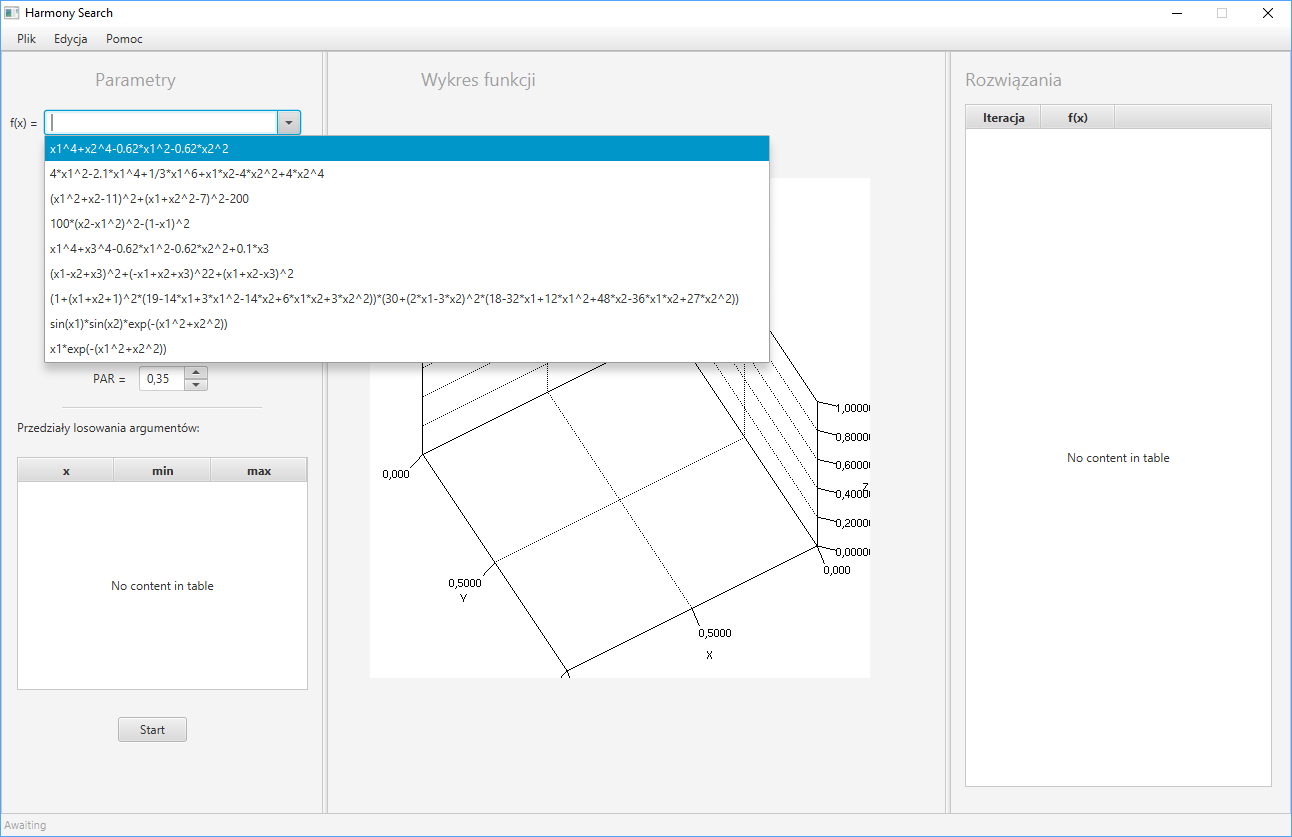
\includegraphics[width=\linewidth]{images/1.PNG} 
		\caption{Wpisywanie funkcji}
		\label{fig:1}
	\end{minipage} 
	\begin{minipage}[b]{.5\linewidth}
		\centering
		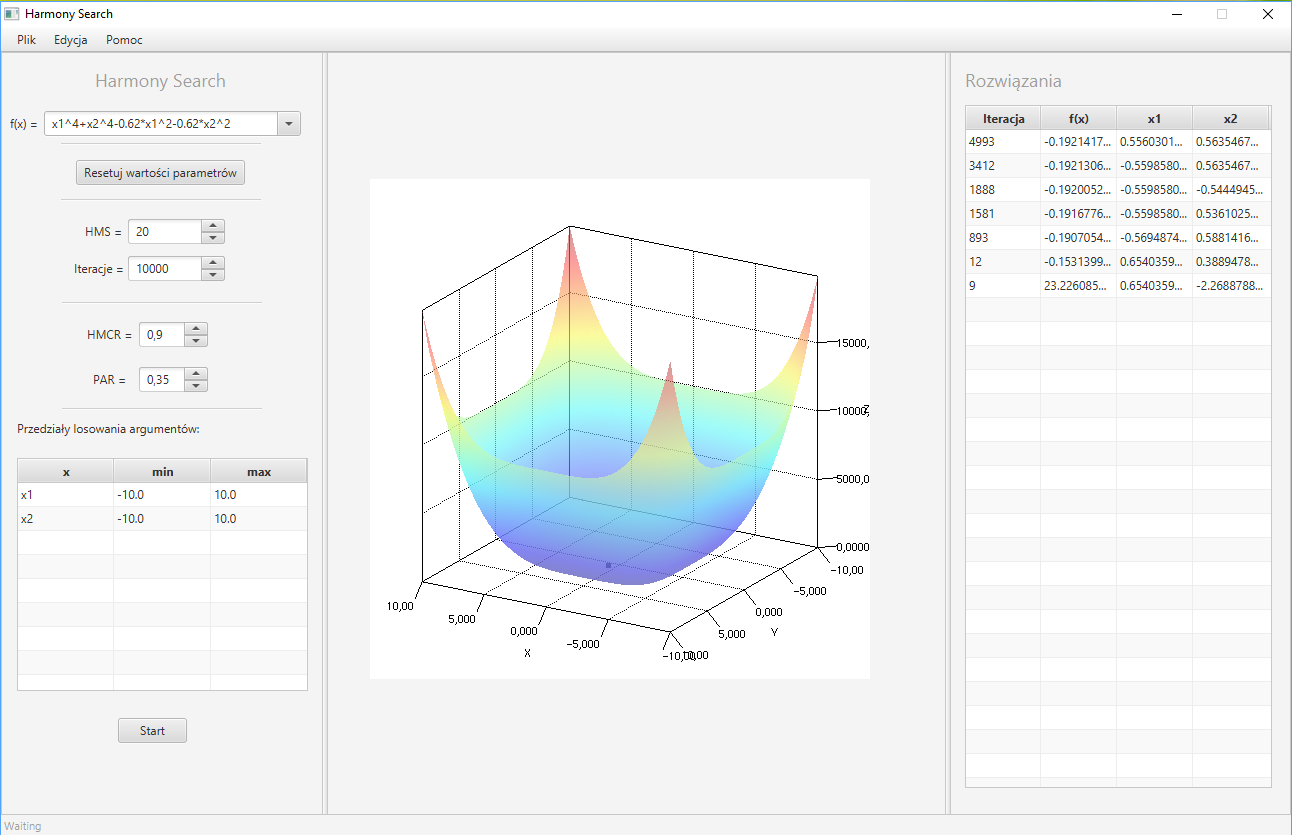
\includegraphics[width=\linewidth]{images/3.PNG} 
		\caption{Wykres z zaznaczonym rozwiązaniem}
		\label{fig:2}
	\end{minipage}
	\newline
	\newline
	\begin{minipage}[b]{1\linewidth}
		\centering
		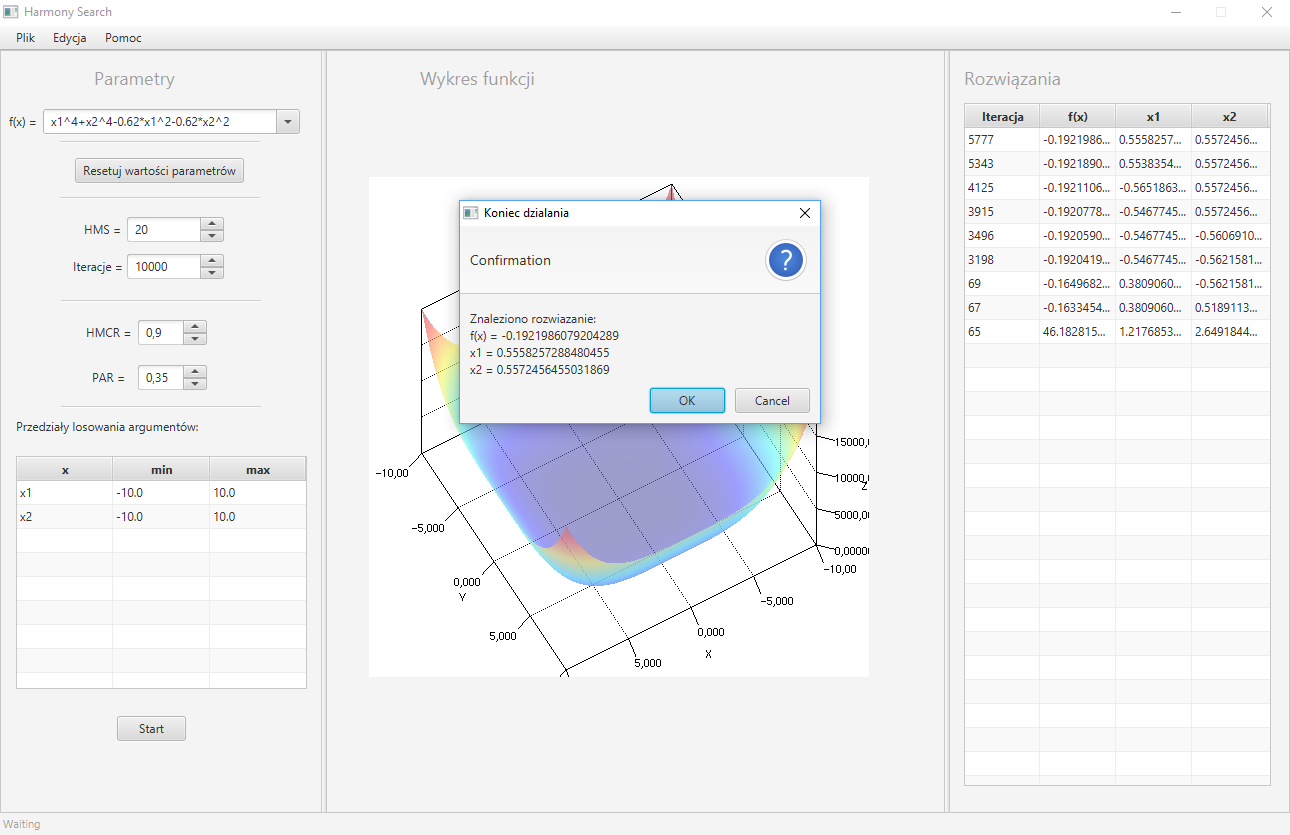
\includegraphics[width=.9\linewidth]{images/2.PNG} 
		\caption{Obliczone rozwiązanie wraz z komunikatem}
		\label{fig:3}
	\end{minipage}
\end{figure}

\subsubsection{Parametry}
\label{subsubsec:parametry}
W części parametrów można dostrzec, że zaraz pod paskiem edycji znajduje miejsce do wpisania funkcji. Jest to ta sama funkcja której minimum należy wyznaczyć. Okno umożliwia również wybór takiej funkcji z wcześniej zadeklarowanych w programie. Dokonuje się tego klikając w rozwijane menu. Zostało to przedstawione na rysunku \ref{fig:1}. Po wybraniu funkcji automatycznie zostaną domyślnie uzupełnione wszystkie parametry obliczeń. Oczywiście możliwa jest dostosowanie algorytmu do własnych potrzeb. Poniżej okna funkcji znajduje się przycisk ,,{\tt Resetuj wartości parametrów}'' umożliwiający, jak mówi nazwa, reset do parametrów domyślnych. Poniżej przycisku zostały umieszczone po sobie cztery główne parametry algorytmu {\em Harmony Search}. \\
Pierwszy z parametrów {\tt HMS} ({\em ang. harmony memory size}) reguluje ilość zapamiętywanych rozwiązań podczas wyszukiwania. Domyślnie rozmiar jest zadeklarowany na $20$. Poniżej znajduje się okno o nazwie {\tt iteracje}. Domyślnie jest zadeklarowana maksymalna wartość iteracji równa $10000$. W każdej iteracji programu algorytm wyszukuje nowe rozwiązanie i sprawdza je z tymi zapisanymi w {\tt HMS}. Czym większa ilość iteracji tym algorytm powinien obliczać dokładniejsze rozwiązanie, kosztem wydłużonego czasu obliczeń. Następnie pod polem {\tt iteracje} znajduje się pole {\tt HMCR} ({\em ang. harmony memory consideration ratio}). Tłumaczenie określa go jako współczynnik wyboru tonu z pamięci. Jest to współczynnik prawdopodobieństwa wybierany z zakresu $(0, 1)$. Czym {\tt HMCR} jest większe tym wyszukiwane wartości {\em x} następnych rozwiązań będą zbliżone do tych istniejących już w tablicy {\tt HMS}. Poniżej znajduje się drugi parametr prawdopodobieństwa dla funkcji o nazwie {\tt PAR} {\em(ang. pitch adjustment ratio)} tłumaczony jako współczynnik dostosowywania tonu. Wybierany jest również z zakresu $(0, 1)$. Na samym dole kolumny znajduje się tabela {\tt Przedziały losowania argumentów}. W tabeli deklarowany jest przedziały wszystkich wartości {\em x} dla których ma być poszukiwane rozwiązanie. Domyślnie parametry dla wszystkich {\em x} brane są z przedziału $(-10, 10)$. Algorytm z dużą dokładnością znajdzie najmniejsze minimum lokalne dla funkcji z podanego przedziału. Po wybraniu wszystkich parametrów można przystąpić do uruchomienia algorytmu przyciskiem {\tt Start} znajdującym się na na dole kolumny.

\subsubsection{Wykres}
\label{subsubsec:wykres}
Środkowy obszar okna głównego przeznaczony jest do wyświetlania wykresu funkcji. Jak wspomniane zostało na początku rozdziału \ref{sec:implementacja}, do rysowania wykresów została użyta zewnętrzna biblioteka {\em jzy3D}. Umożliwia ona tworzenie wykresów dwu i trzy wymiarowych.  Wykresy można obracać w dowolny sposób. Oś {\em X} i {\em Y} wykresu wyskalowana jest do najmniejszego i największego parametru wszystkich wartość {\em x}. Dodatkowo wartości zostały pokolorowane w tak, że mniejsze wartości funkcji mają kolory zimniejsze, a wyższe kolory cieplejsze, analogicznie do tego jak przedstawia się wysokość n.p.m. w kartografii. Dodatkowo czarną kropką zaznaczona została najmniejsza obliczona wartość funkcji. 

\subsubsection{Tabela Rozwiązań}
\label{subsubsec:rozwiazania}
Po prawej stronie okna głównego można dostrzec najlepsze rozwiązania wyszukane przez program. Gdy znajdowane jest rozwiązanie lepsze od najlepszego rozwiązania zapamiętanego w {\tt HMS} dodawane jest ono jako pierwszy wiersz w tabeli. Poprzednie rozwiązania przesuwane są o jedno miejsce niżej. Pozwala to śledzić jaka wartości jest aktualnie największa oraz od razu ukazuje się obok numer iteracji tego rozwiązania. Gdy algorytm długo oblicza najlepszy wynik okno pozwala śledzić postęp obliczeń. Dodatkowo po wykonaniu wszystkich iteracji zostaje wyświetlony komunikat z najlepszym rozwiązaniem (pierwszym od góry), co przedstawia rysunek \ref{fig:3}.

\subsection{Pliki}
\label{subsec:pliki}
Program był pisany w środowisku programistycznym {\em IntelliJ IDEA}. Jak wcześniej wspomniano do stworzenia GUI programu użyto technologii {\em JavaFx} umożliwiającej tworzenie aplikacji okienkowych. Dodatkowo by ułatwić zarządzanie bibliotekami wewnątrz programu użyto wsparcia ze strony {\em Maven}. By ułatwić zrozumienie tekstu stworzono graficzną wersję struktury plików i katalogów. Główny kod programu został umieszczony katalogu {\tt src}. Katalog zawiera w sobie dwa inne katalogi {\tt resourses} oraz {\tt java}. Katalog {\tt resourses} posiada jeden folder w którym umieszczony jest plik {\tt main.fxml} odpowiedzialny GUI programu. W tym pliku zapisane są informacje o ułożeniu i wielkości elementów, które widzi użytkownik. Można powiedzieć że plik odpowiada za foreground programu. \\
Cała background programu czyli jego mechanika jest umieszczona w folderze {\tt java}. Posiada on dwa podfoldery {\tt org.jzy3d} oraz {\tt com.blag.harmonysearch}. Pierwszy katalog odpowiedzialny jest za generowanie wykresów w oknie opisywanym w rozdziale \ref{subsubsec:wykres}. Są to pliki zewnętrzne pobrane ze strony \cite{bib:jzy3d}. Katalog {\tt com.blag.harmonysearch} zawiera cztery foldery. Każdy z nich posiada pliki napisane na potrzeby tego projektu. Dla czytelności opisu zostaną one przedstawione jako kolejne podrozdziały. 

\subsubsection{Katalog {\tt contants}}
\label{subsubsec:contants}
W tym katalogu zadeklarowane są tylko dwa pliki. W pliku {\tt DefaultFunctionStrings} zadeklarowano przykładowe funkcję wspominane w \ref{subsubsec:parametry}. Plik {\tt HarmonySearchConstans} odpowiada za domyślne parametry. 

\subsubsection{Katalog {\tt core}}
\label{subsubsec:core}
W katalogu {\tt core} znajdują się najważniejsze pliki odpowiedzialne za działanie programu. Klasa {\tt ArgumentGenerationRules} jest klasą przechowującą zasady generowania argumentów. Klasa {\tt ArgumentLimit} implementuje zakres z jakiego wyszukiwane będą elementy. Główną klasą gdzie przechowywane są wartości jest klasa {\tt HarmonyMemory}. Posiada ona tablice rozwiązań, której wielkość jest regulowana z GUI programu. Tablica w została zaimplementowana jako {\tt SortedSet} co ogromnie przyspiesza przeszukiwanie. Klasą gdzie zadeklarowany jest główny algorytm czyli gdzie wykonywane są operacje obliczeń jest klasa {\tt HarmonySearcher}. Wylosowane rozwiązanie przekazywane jest jako lista złożona z typu {\tt Solution}. Klasa {\tt SolutionGenerator} umożliwia wygenerowanie nowych wartości {\em x} dla którego zostanie obliczone rozwiązanie. Ostatnia klasa w tym pliku {\tt SolutionValueComparator}, porównuje czy rozwiązanie dla wylosowanych {\em x} jest lepsze od rozwiązań zadeklarowanych w tablicy. 
\\
\begin{forest}
	for tree={font=\tt, grow'=0, folder icons, edge=densely dotted}
	[/src/main/
	[\ \ java
	[\ \ com.blag.harmonysearch
	[\ \ contans
	[     DefaultFunctionStrings, is file]
	[     HarmonySearchConstans, is file]]
	[\ \ core
	[     ArgumentGenerationRules, is file]
	[     ArgumentLimit, is file]
	[     HarmonyMemory, is file]
	[     HarmonySearcher, is file]
	[     Solution, is file]
	[     SolutionGenerator, is file]
	[     SolutionValueComparator, is file]]
	[\ \ gui
	[     Controller, is file]
	[     HarmonySearcherGui, is file]
	[     Main, is file]
	[     Plot, is file]
	[     SolutionGui, is file]]
	[\ \ helpers
	[     ArgumentMatching, is file]
	[     BoundedTreeSet, is file]
	[     Extensions, is file]
	[     FunctionStringValidator, is file]
	[     RandomGenerator, is file]]]
	[ \ \ org.jzy3d
	[(...),is file]]]
	[ \ \ resources
	[ \ \ fxml
	[     main.fxml, is file]]]]
\end{forest}
\newline

\subsubsection{Katalog {\tt gui}}
\label{subsubsec:gui}
W katalogu znajdują się klasy odpowiedzialne za kontrolowanie tego co ma wypisać bądź wyrysować się na ekranie. Katalog {\tt Controller} dostarcza bezpośrednio wartości do pliku {\tt main.fxml}. Do obliczeń pobiera wartości z klasy {\tt HarmonySearcherGui}. Klasa {\tt Main} aktywowana jest po rozpoczęciu pracy programu jako pierwsza i pobudza całość programu do działania. Wykres tworzony jest dzięki obiektowi klasy {\tt plot}, a w obiekcie klasy {\tt SolitionGui} wyświetlane są wyniki. Klasy {\tt Gui} są rozszerzeniem klas z folderu {\tt core} opisanych w \ref{subsubsec:core}.

\subsubsection{Katalog {\tt helpers}}
\label{subsubsec:helpers}
Katalog zawiera głównie klasy pomocne będące rozszerzeniem klas podstawowych {\em Javy}. Klasy rozwijają Listy, drzewa, generatory i wiele innych klas o funkcjonalności niezbędne do działania programu. Zostały wykorzystane jako wsparcie w implementacji w plikach z katalogu {\tt core}.

\section{Przykładowy rozwiązań oraz testy}
\label{sec:przyklady}
W tej części zostały przedstawione trzy przykłady funkcji dwóch zmiennych {\em $x_{1}$} i {\em $x_{2}$} wraz z obliczonymi rozwiązaniami.

\subsection{Funkcja czterech minimum}
\label{subsec:fcn4min}
Pierwsza zostanie przedstawiona funkcja posiadająca cztery minima lokalne. Posiada ona następujący wzór: $$f(x_{1},x_{2}) = x_{1}^{4}+x_{2}^{4}-0.62x_{1}^{2}-0.62x_{2}^{2} $$.  Rysunek \ref{fig:11} prezentuje trójwymiarowy wykres funkcji na przedziale $x_{1}, x_{2} \in <-1,1>$ wraz z zaznaczoną najmniejszą obliczoną wartością $f(-0.56,56)=-0.19$. Dokładną wartość $10^(-15)$ można odczytać po prawej stronie w tabeli {\tt Rozwiązania}i. 
\begin{figure}[htbp]
	\centering
		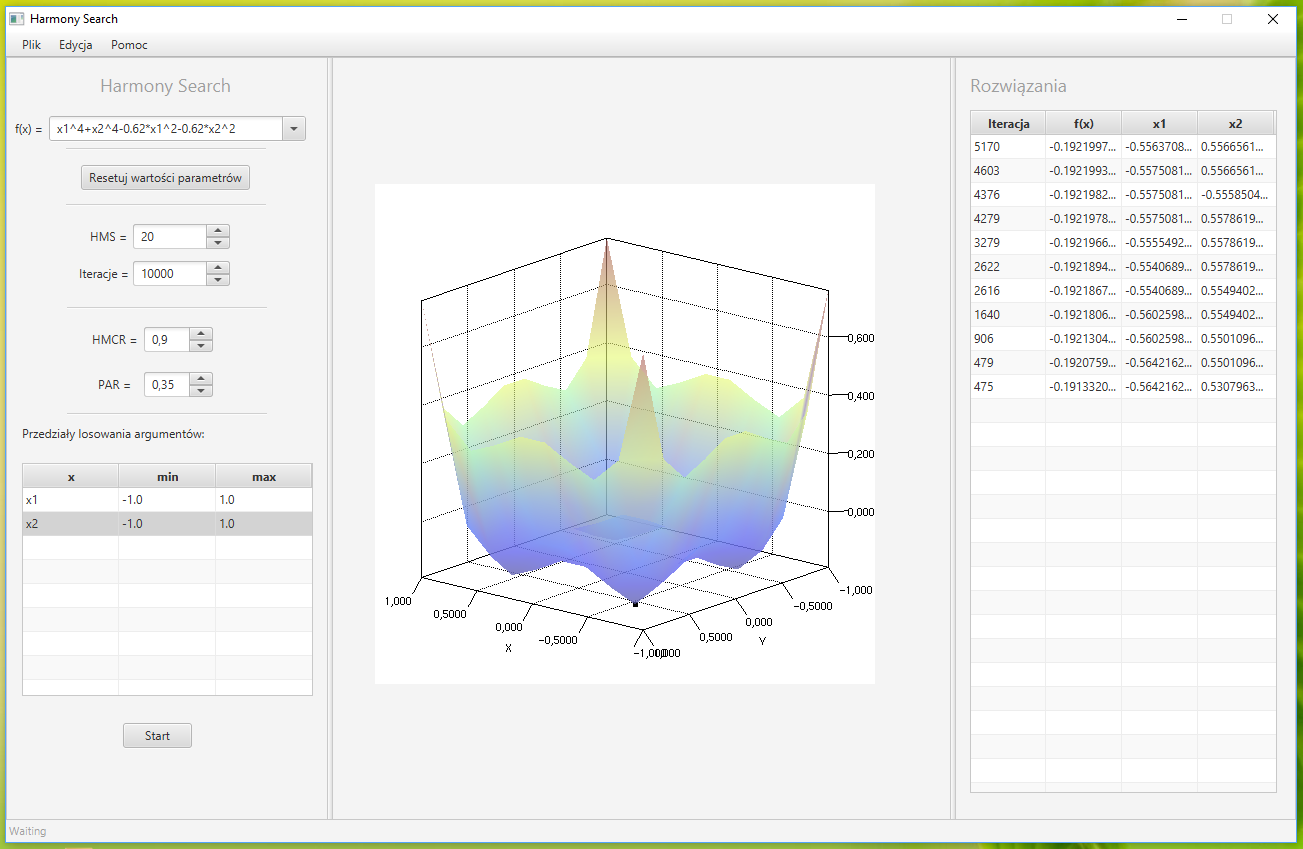
\includegraphics[width=.9\textwidth]{images/11.PNG}
		\caption{Wykres funkcji czterech minimum $x_{1}, x_{2} \in <-1,1>$}
		\label{fig:11}
\end{figure}
\subsubsection{Zmiana zakresu dla argumentów}
\label{subsubsec:fcn4min2}
By wyznaczyć wartość interesującego nas minimum należy zawęzić przedział. Przypadki prezentowane na rysunkach \ref{fig:12}, kolejno pokazują wszystkie minima zależnie od podanego przedziału. Jak możemy dostrzec na wykresach algorytm znalazł rozwiązanie na każdym przedziale.
\begin{figure}[htbp] 
	\begin{minipage}[b]{.5\textwidth}
		\centering
		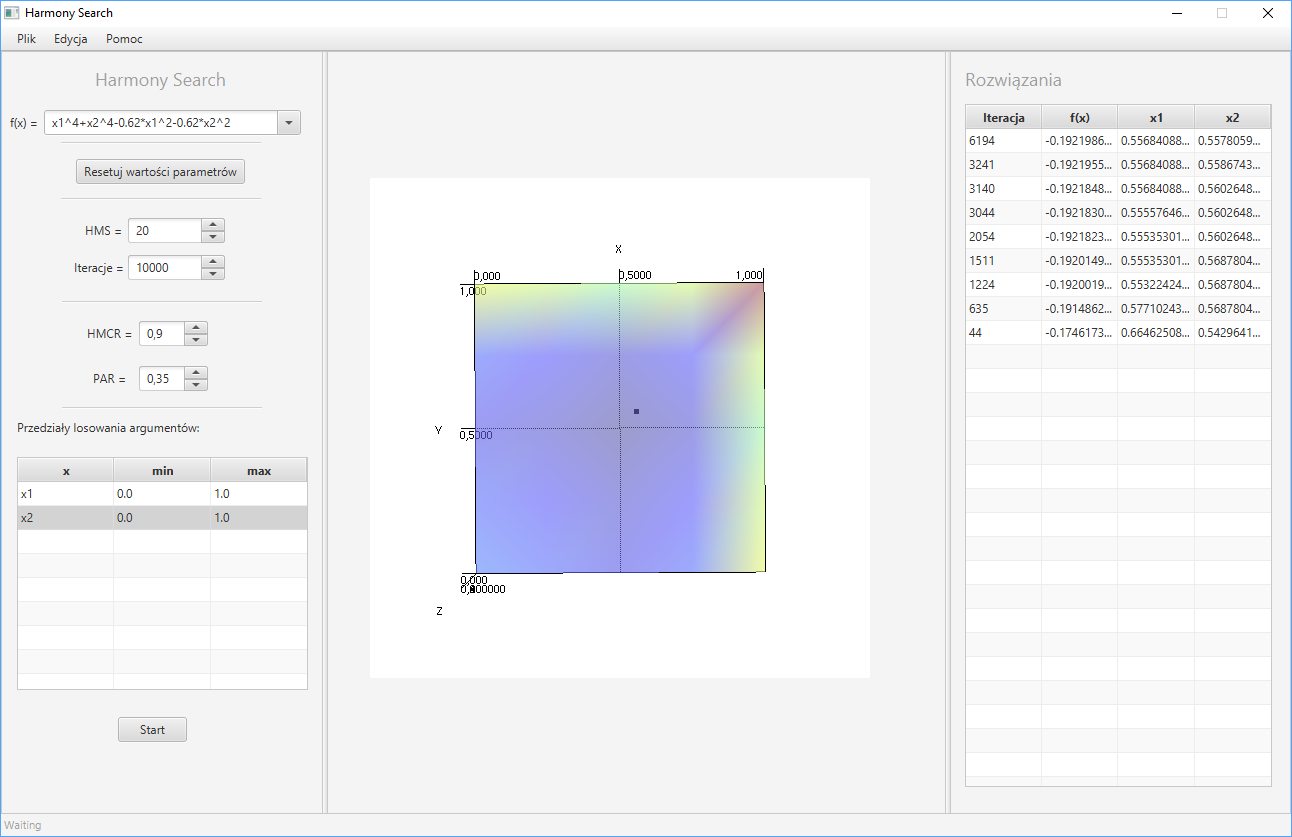
\includegraphics[width=\linewidth]{images/12.PNG}
		\caption{$x_{1}\in<0,1>,  x_{2}\in<0,1>$}
	\end{minipage} 
	\begin{minipage}[b]{.5\textwidth}
		\centering
		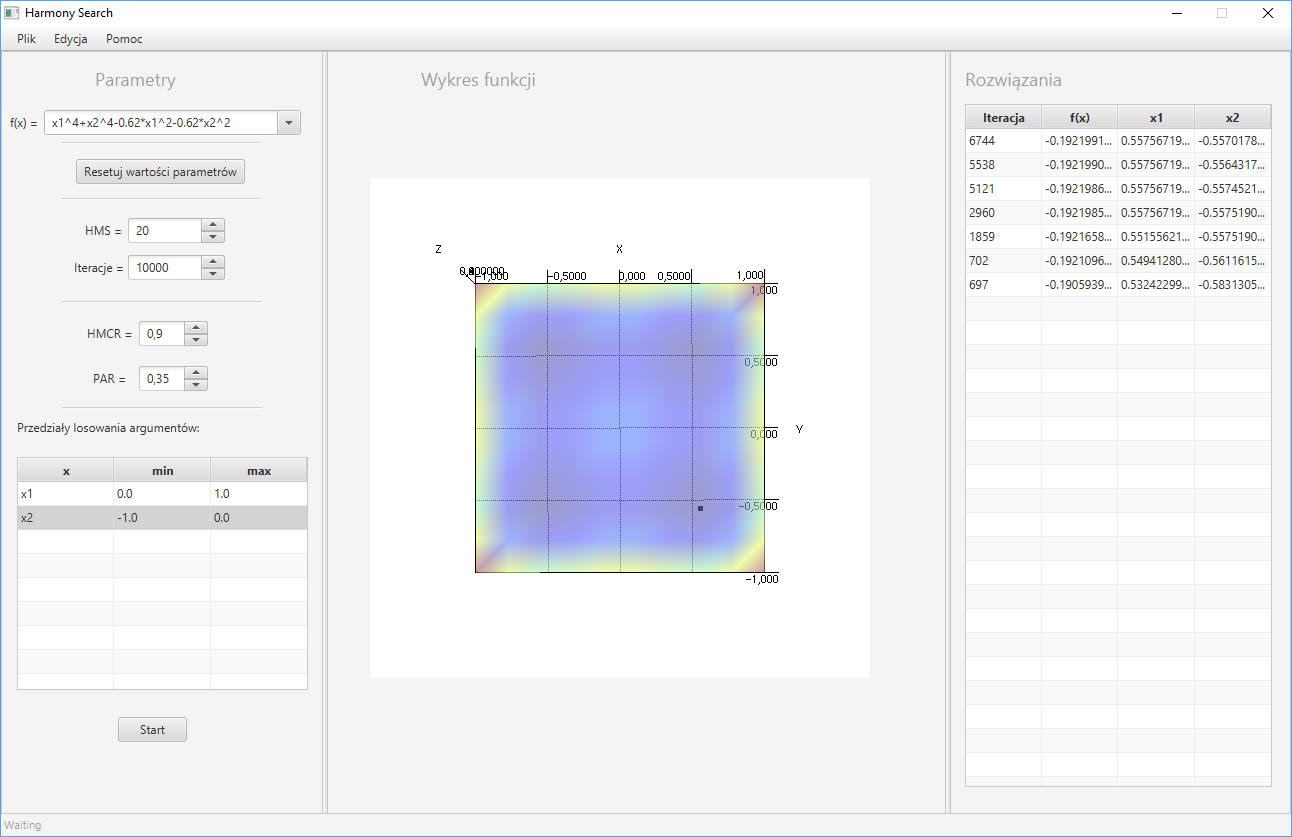
\includegraphics[width=\linewidth]{images/17.PNG} 
		\caption{$x_{1}\in<0,1>,  x_{2}\in<-1,0>$}
	\end{minipage}
	\newline \newline
	\begin{minipage}[b]{.5\textwidth}
		\centering
		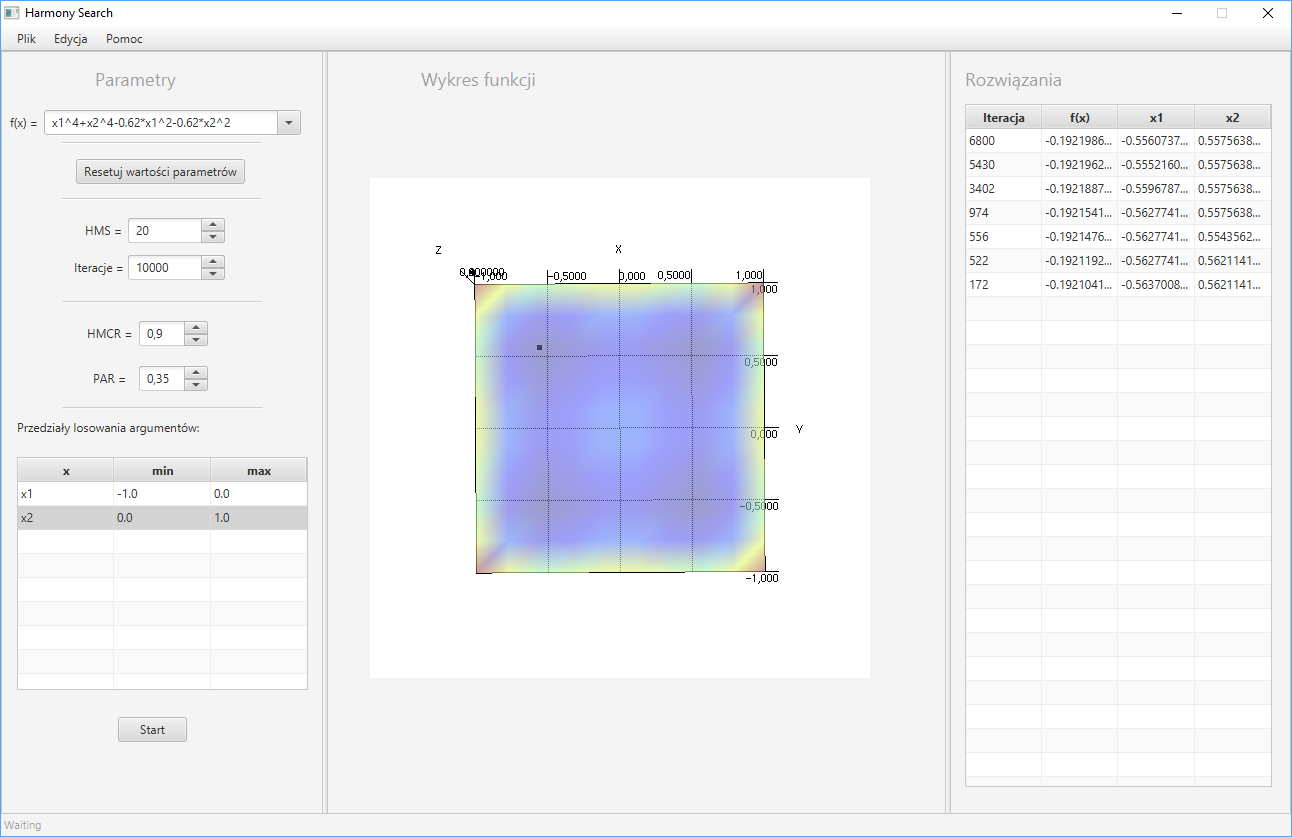
\includegraphics[width=\linewidth]{images/16.PNG}
		\caption{$x_{1}\in<-1,0>,  x_{2}\in<0,1>$}
	\end{minipage} 
	\begin{minipage}[b]{.5\textwidth}
		\centering
		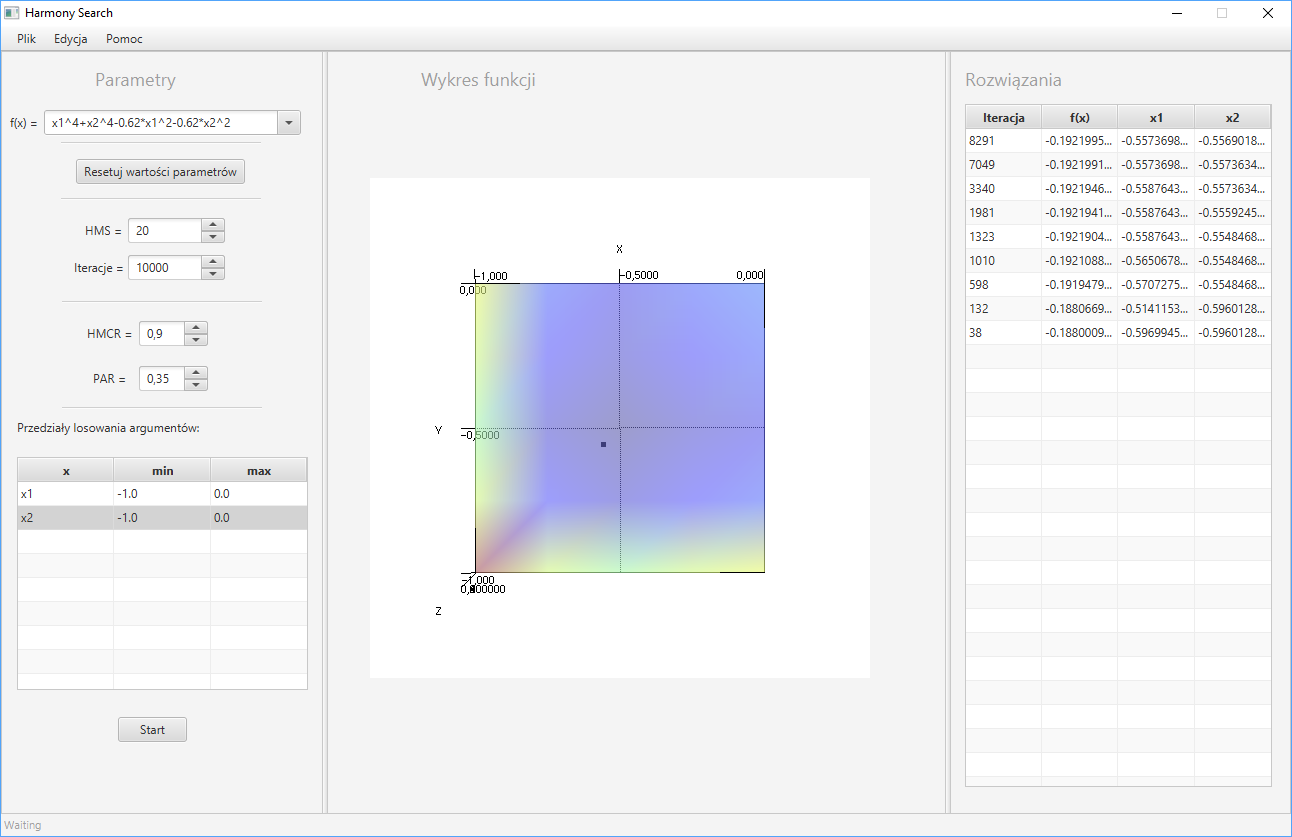
\includegraphics[width=\linewidth]{images/14.PNG}
		\caption{$x_{1}\in<-1,0>,  x_{2}\in<-1,0>$}
	\end{minipage}
	\label{fig:12}
	\caption{Wykres funkcji czterech minimum dla różnych przedziałów}
\end{figure}
 
\subsection{Funkcja Gemm}
\label{subsec:gemm}
Kolejny przykład przedstawiał funkcję opisaną równaniem $$f(x_{1},x_{2}) = x_{1}^{4}+x_{2}^{4}-0.62x_{1}^{2}-0.62x_{2}^{2}$$. Początkowo zakres dla argumentów funkcji został przyjęty jako $x_{1},x_{2} \in <-0.5,1>$. Wykres funkcji wraz z rozwiązaniem zaprezentowany jest na \ref{fig:21}. 
\begin{figure}[htbp]
	\centering
	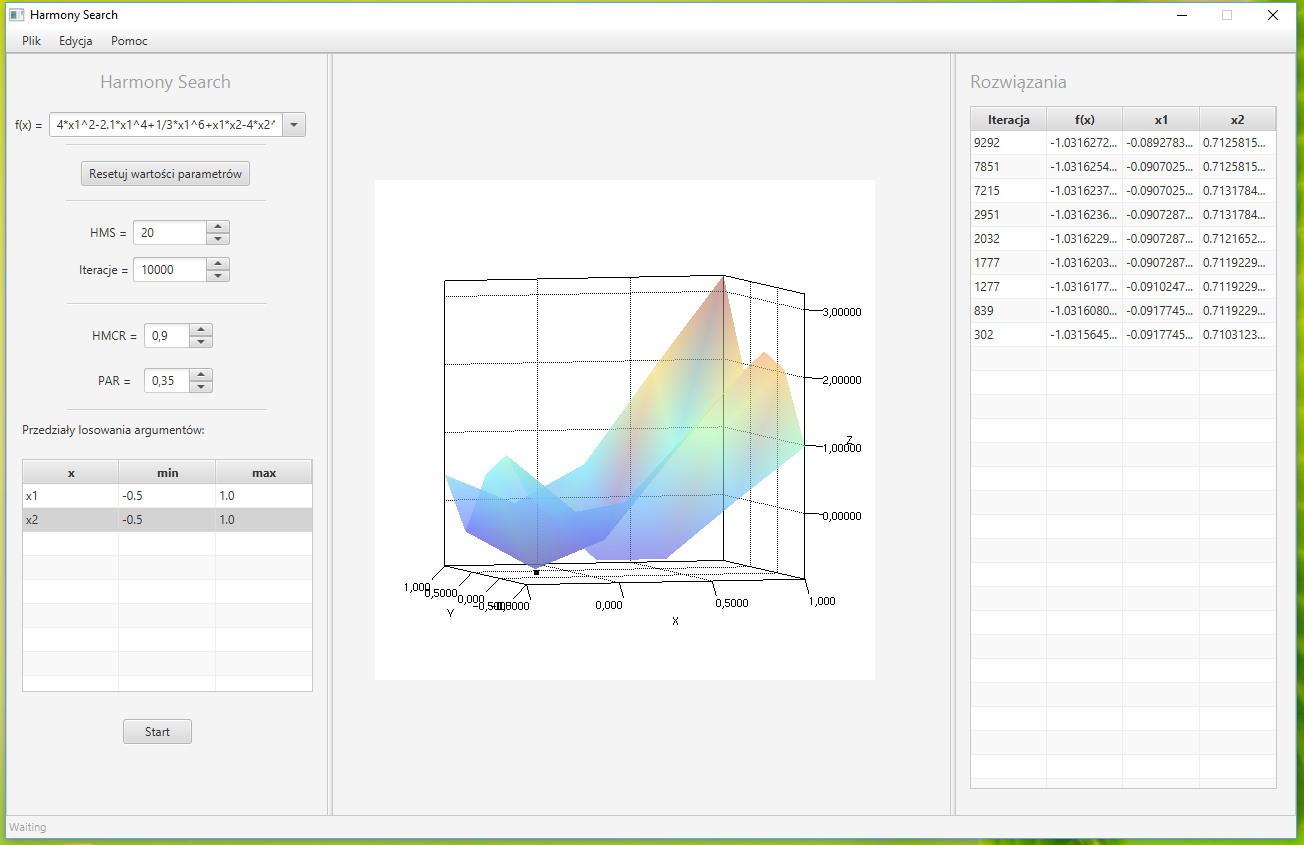
\includegraphics[width=.9\textwidth]{images/21.PNG}
	\caption{Wykres funkcji Gemm dla $x_{1}, x_{2} \in <-0.5,1>$}
	\label{fig:21}
\end{figure}

\subsubsection{Zmiana zakresu dla argumentów}
\label{subsubsec:gemm2}
Jak w poprzednim przykładzie tak i tutaj postanowiono zmienić zakres wyszukiwania argumentów na $x_{1}, x_{2} \in <-2,2>$. Porównując oba rozwiązania można stwierdzić, że odnalezione punkty nie różnią się zbytnio.  
\begin{figure}[htbp] 
	\begin{minipage}[b]{.5\textwidth}
		\centering
		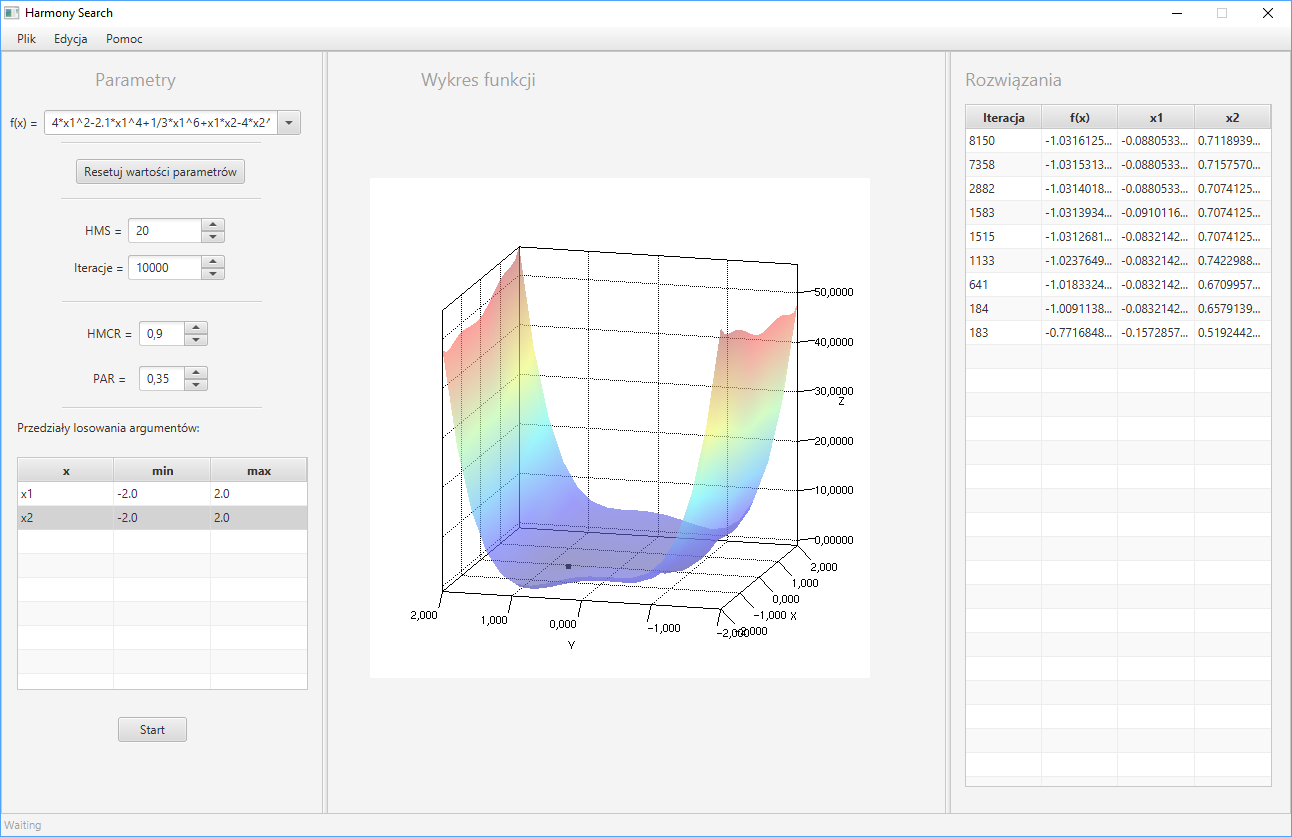
\includegraphics[width=\linewidth]{images/22.PNG} 
	\end{minipage} 
	\begin{minipage}[b]{.5\textwidth}
		\centering
		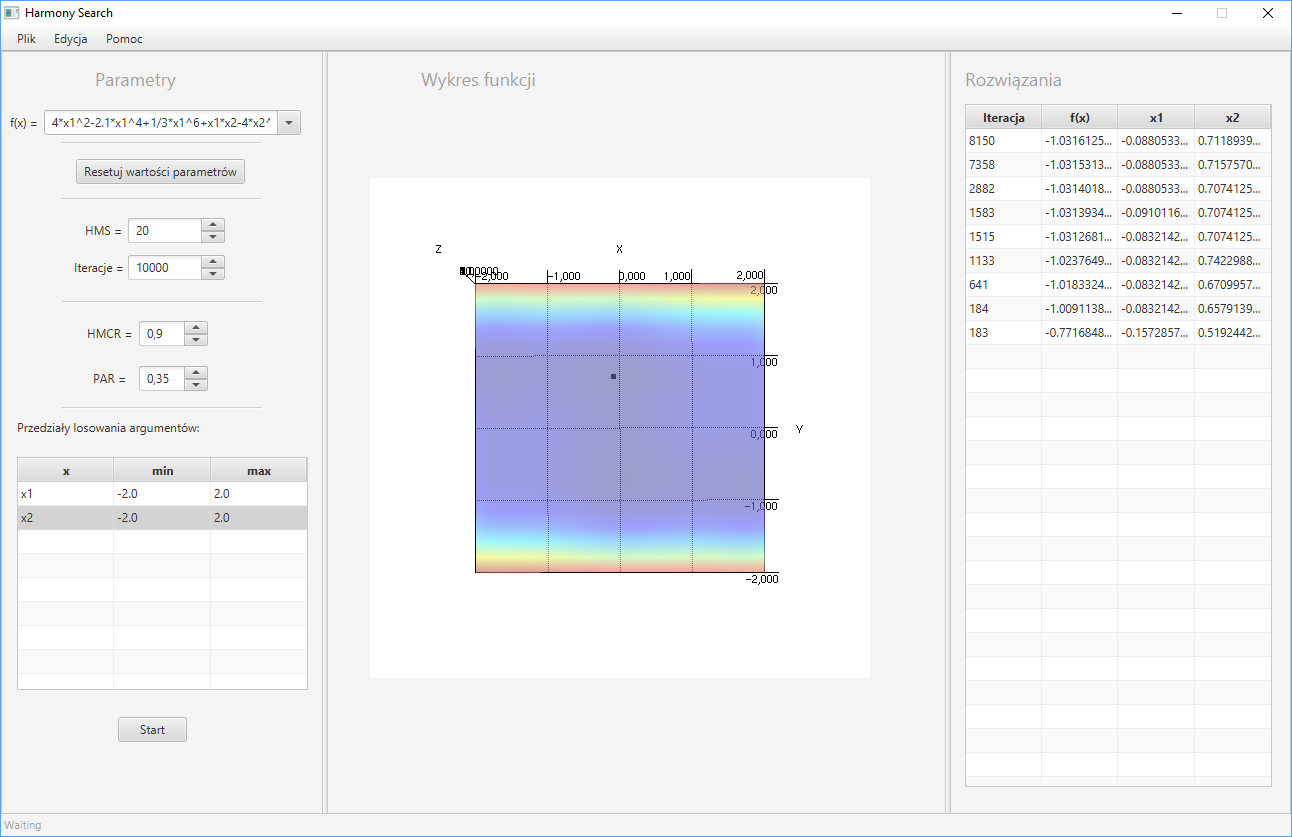
\includegraphics[width=\linewidth]{images/23.PNG} 
	\end{minipage}
	\label{fig:22}
	\caption{Wykresy funkcji Gemm dla $x_{1}, x_{2} \in <-2,2>$}
\end{figure}

\subsection{Funkcja Himmelblau}
\label{subsec:himmelblau}
Funkcja Himmelbalu również jak \ref{subsec:fcn4min} posiada cztery minima lokalne zlokalizowane po jednym w każdej ćwiartce na przedziale $x_{1,2} \in (-5,5)$. Funkcja posiada wzór: $$ f(x_{1},x_{2}) = (x_{1}^{2}+x_{2}-11)^{2}+(x_{1}+x_{2}^{2}-7)^{2}-200$$. Dla pokazania, że funkcja wyszukuje rozwiązania z innego przedziału jak domyślny ograniczono się do przedziału z pierwszej ćwiartki $x_{1}, x_{2} \in (0,10)$. Na wykresie \ref{fig:5} zaprezentowany został wykres funkcji wraz z naniesionym najlepszym rozwiązaniem. 
\begin{figure}[htbp] 
	\begin{minipage}[b]{.5\textwidth}
		\centering
		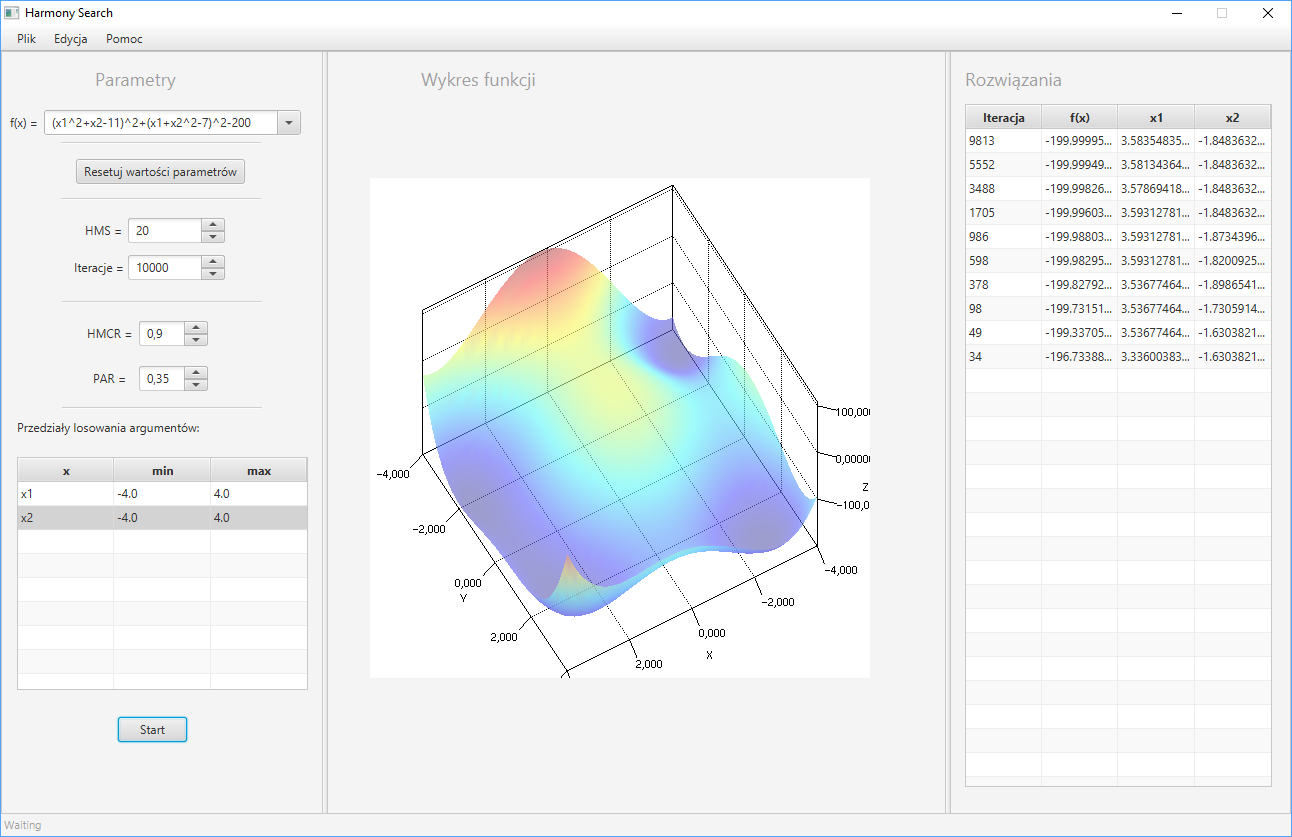
\includegraphics[width=\linewidth]{images/31.PNG} 
	\end{minipage} 
	\begin{minipage}[b]{.5\textwidth}
		\centering
		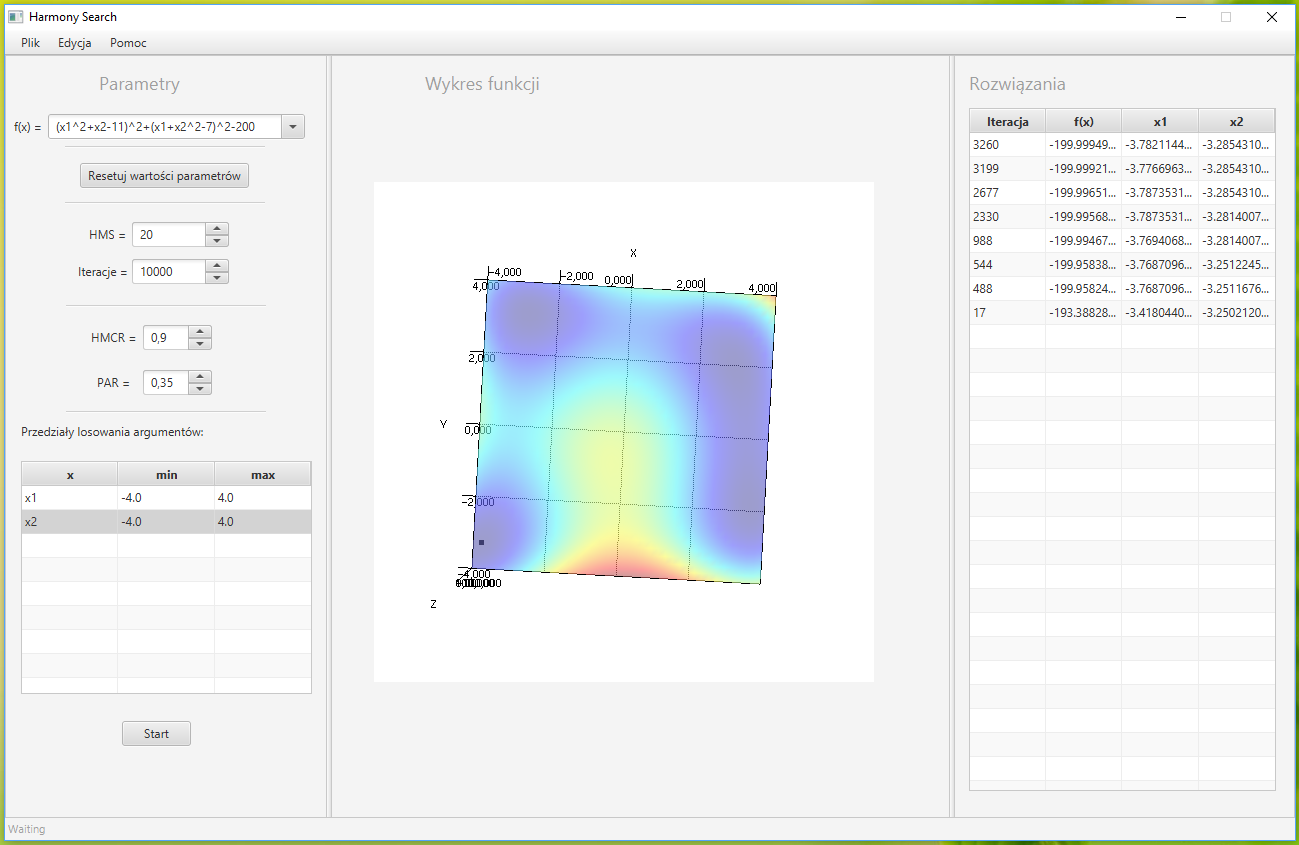
\includegraphics[width=\linewidth]{images/32.PNG} 
	\end{minipage}
	\label{fig:31}
	\caption{Wykresy funkcji Himmelblau dla $x_{1}, x_{2} \in <-4,4>$}
\end{figure}

\subsection{Funkcja trzech zmiennych}
\label{subsec:trzyzmienne}
By przetestować działanie programu i algorytmu dla funkcji z trzema zmiennymi wybrano funkcję $$f(x_{1},x_{2},x_{3}) = x_{1}^{4}+x_{3}^{4}-0.62x_{1}^{2}-0.62x_{2}^{2}+0.1x_{3}$$. Oczywistym jest, że wykres czterowymiarowy jest niemożliwy do wyrysowania dlatego okno wykresu zostało puste co prezentuje \ref{fig:41}. W tysięcznej iteracji obliczono minimalną wartość funkcji $f(-3.43,-7171,1.58)=-3.19$. Można się spodziewać, że w kolejnych iteracjach znaleziona by była mniejsza wartość minimalna lecz ograniczenie spowodowało zatrzymacie cyklu obliczeń. W takim przypadku najlepszym rozwiązaniem jest zmniejszenie obszaru dla zmiennych $x$.
\begin{figure}[htbp]
	\centering
	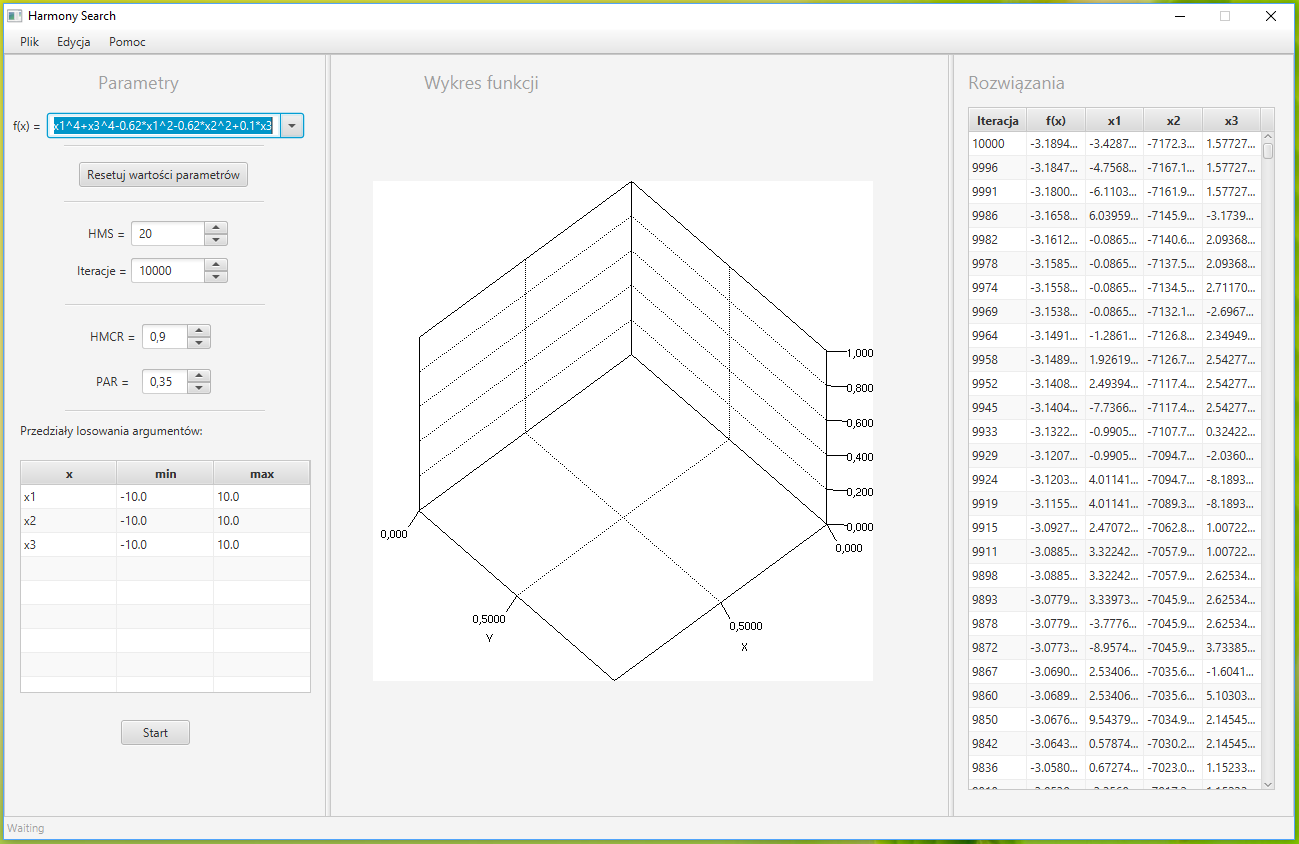
\includegraphics[width=.6\textwidth]{images/41.PNG}
	\caption{Wykres funkcji trzech zmiennych $x_{1}, x_{2}, x_{3} \in <-10,10>$}
	\label{fig:41}
\end{figure}

\subsection{Funkcja ceny złota}
\label{subsec:cenyzlota}
Funkcja Ceny złota \cite{bib:goldstein} posiada kilka minimów lokalnych umiejscowionych blisko siebie. Opisuje ją jeden z dłuższych wzorów $$f(x_{1},x_{2}) = (1+(x_{1}+x_{2}+1)^2*(19-14x_{1}+3x_{1}^2-14x_{2}+6x_{1}x_{2}+3x_{2}^2))* (30+(2x_{1}-3x_{2})^2*(18-32x_{1}+12x_{1}^2+48x_{2}-36x_{1}x_{2}+27x_{2}^2))$$. Wpierw na rysunku \ref{fig:71} ostało przedstawione rozwiązanie dla  $x_{1}, x_{2} \in <-3,3>$. Następnie na rysunku \ref{fig:72} zakres został zmieniony na $x_{1}, x_{2}, x_{2} \in <-2,0>$. Zarówno dla jednego jak i drugiego zakresu program obliczył właściwe rozwiązanie. 
\begin{figure}[htbp] 
	\begin{minipage}[b]{.5\textwidth}
		\centering
		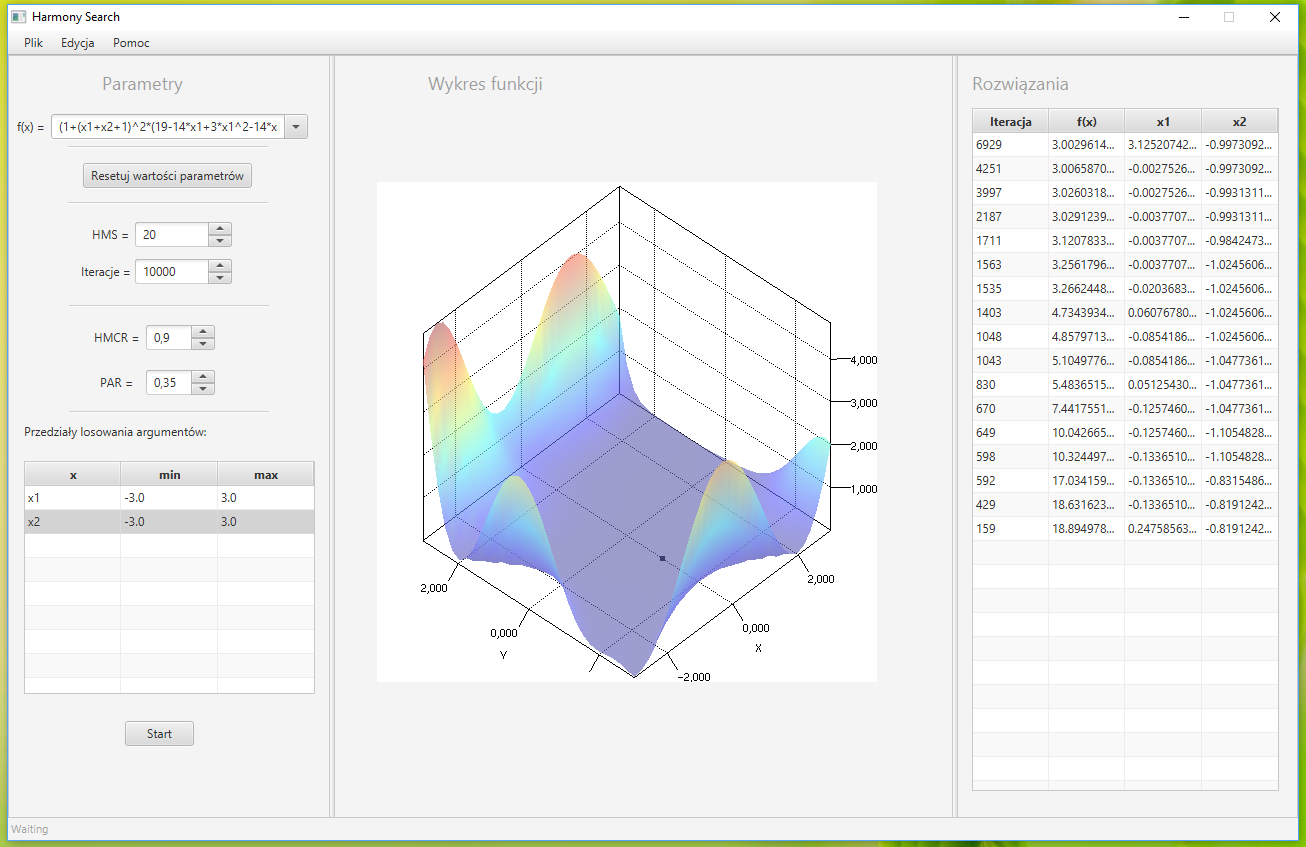
\includegraphics[width=\linewidth]{images/71.PNG}
		\label{fig:71}
		\caption{Wykres ceny złota dla \newline $x_{1},x_{2}\in<-3,3>$}
	\end{minipage} 
	\begin{minipage}[b]{.5\textwidth}
		\centering
		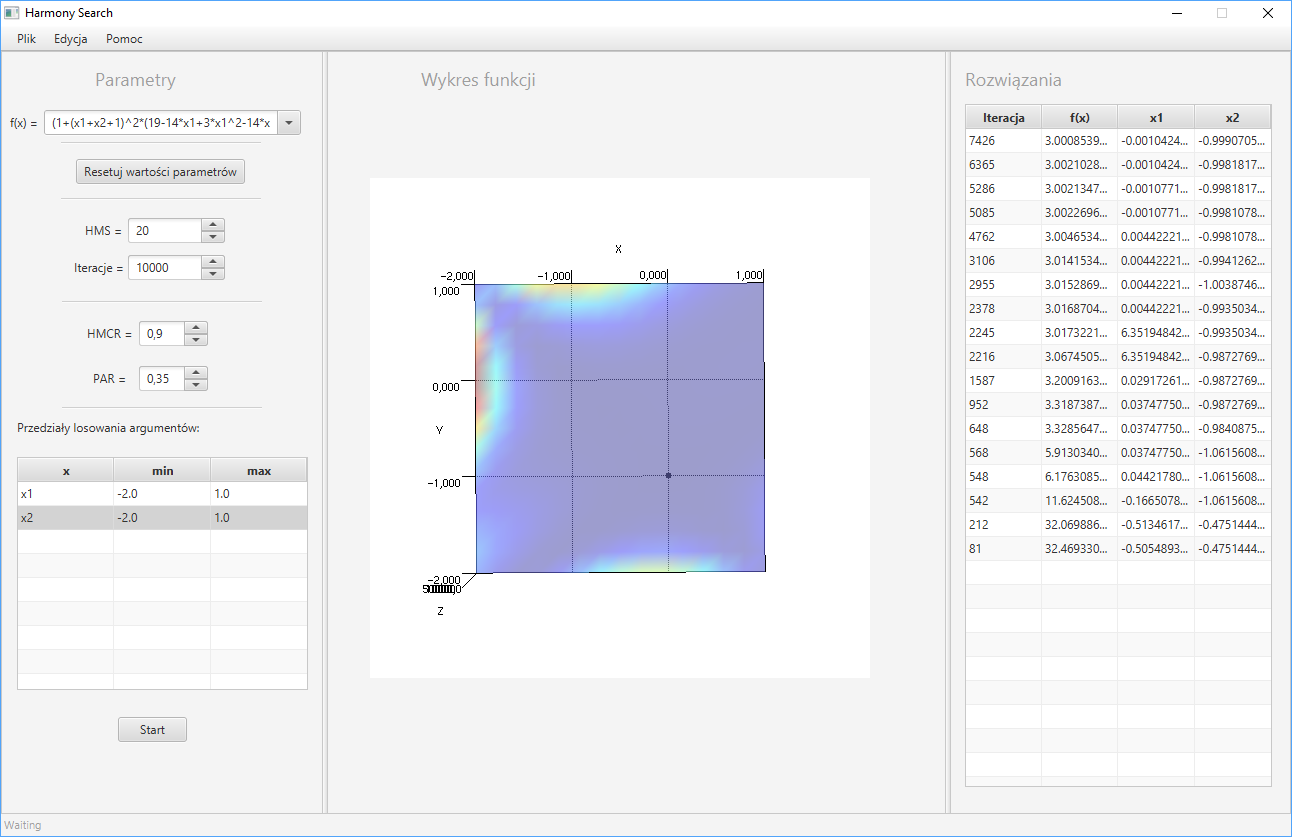
\includegraphics[width=\linewidth]{images/72.PNG} 
		\label{fig:72}
		\caption{Wykres ceny złota dla \newline $x_{1}, x_{2} \in <-2,0>$}
	\end{minipage}
\end{figure}

\subsection{Dwuwymiarowa funkcja sinusoidalna}
\label{subsec:sin}
Dwuwymiarowa funkcja sinus posiada bardzo zróżnicowany przebieg oraz wiele równoważnych minimów lokalnych. Wzór funkcji przedstawiony jest równaniem $$f(x_{1},x_{2})=\sin{x_{1}}\sin{x_{2}}e^{-(x_{1}^2+x_{2}^2)}$$. Rysunek \ref{fig:8} prezentuje wykres funkcji dla argumentów z przedziału $<-1,1$.
\begin{figure}[htbp] 
	\begin{minipage}[b]{.5\textwidth}
		\centering
		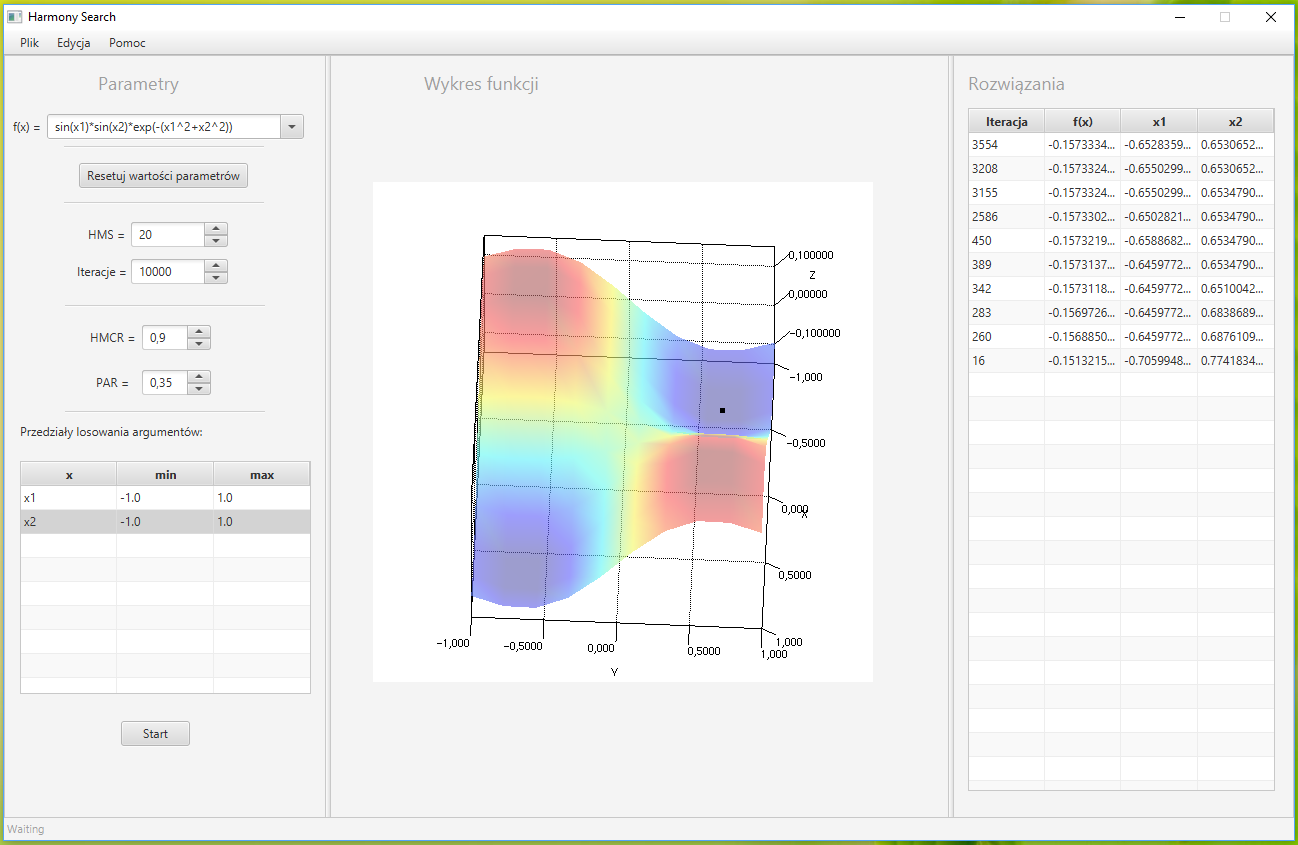
\includegraphics[width=\linewidth]{images/81.PNG}
	\end{minipage} 
	\begin{minipage}[b]{.5\textwidth}
		\centering
		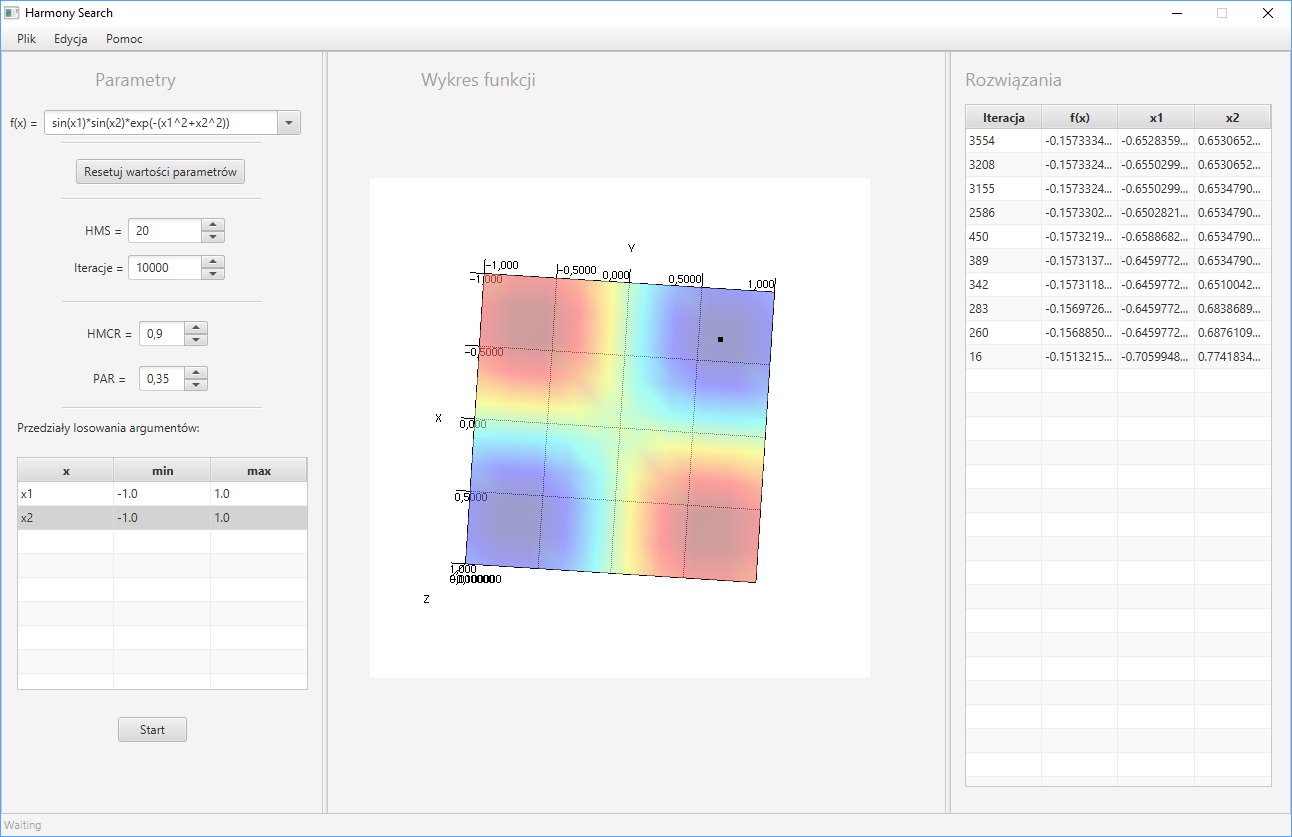
\includegraphics[width=\linewidth]{images/82.PNG} 
	\end{minipage}
	\label{fig:8}
	\caption{Wykres funkcji sinus dla $x_{1}, x_{2} \in <-1,1>$}
\end{figure}

\subsection{Dwuwymiarowa funkcja sinusoidalna z eksponentom}
\label{subsec:sinexp}
Ostatnia przedstawiana funkcja ukazuje przypadek połączenia funkcji sinusa-cosinusa z eksponent. Przypadek jest o tyle ciekawy, że większość wartości funkcji jest dla {\em $x_{1}, x_{2}$} jest do siebie zbliżona. Blisko jej wartość ulega dużemu odchyłowi.  Wzór funkcji przedstawiony jest jako: $$f(x)=x_{1}e^{-(x_{1}^{2}+x_{2}^2)}$$. Rysunek \ref{fig:9} prezentuje działanie programu z obliczoną wartością minimalną. Jak możemy dostrzec program dobrze wyliczył jej wartość co potwierdza jego odporność na działanie funkcji, dla której większość argumentów jest stała. 
\begin{figure}[htbp] 
	\begin{minipage}[b]{.5\textwidth}
		\centering
		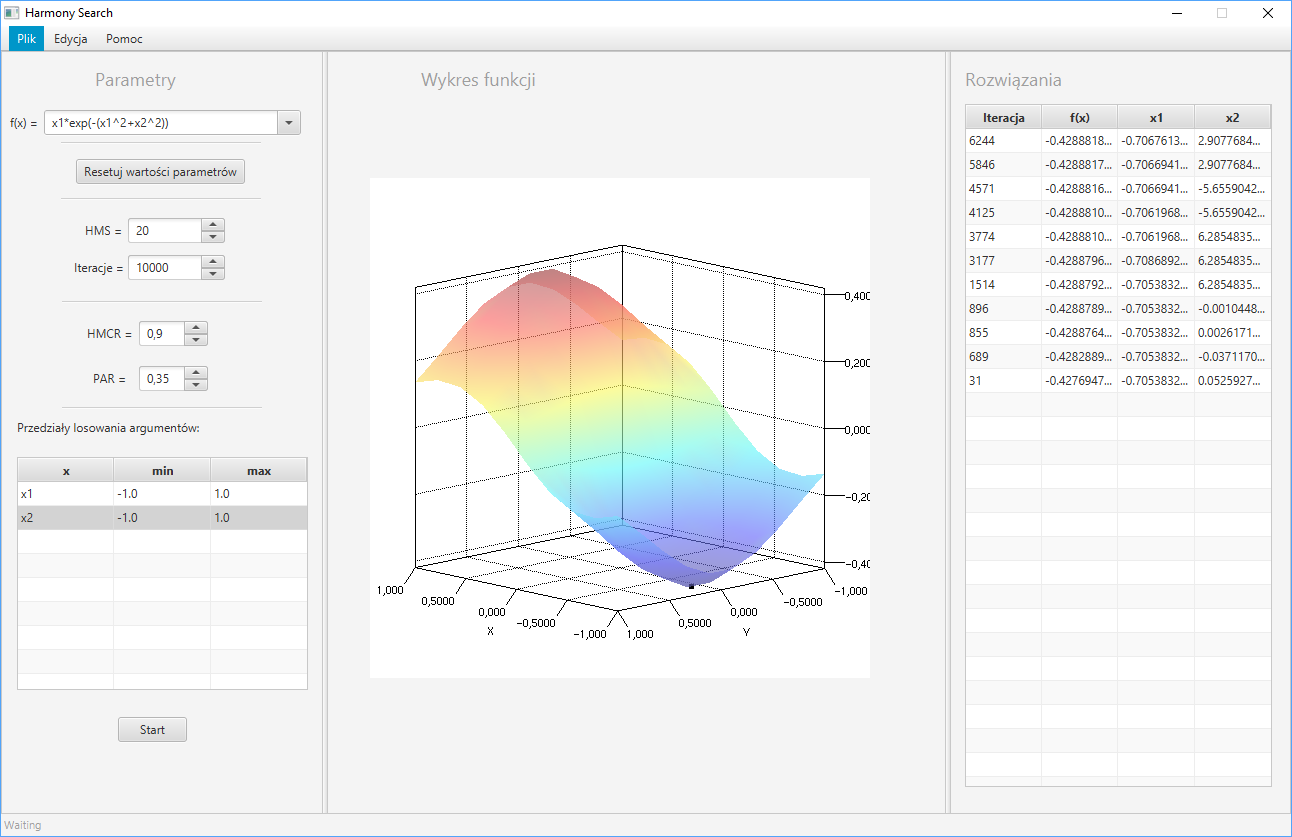
\includegraphics[width=\linewidth]{images/91.PNG}
	\end{minipage} 
	\begin{minipage}[b]{.5\textwidth}
		\centering
		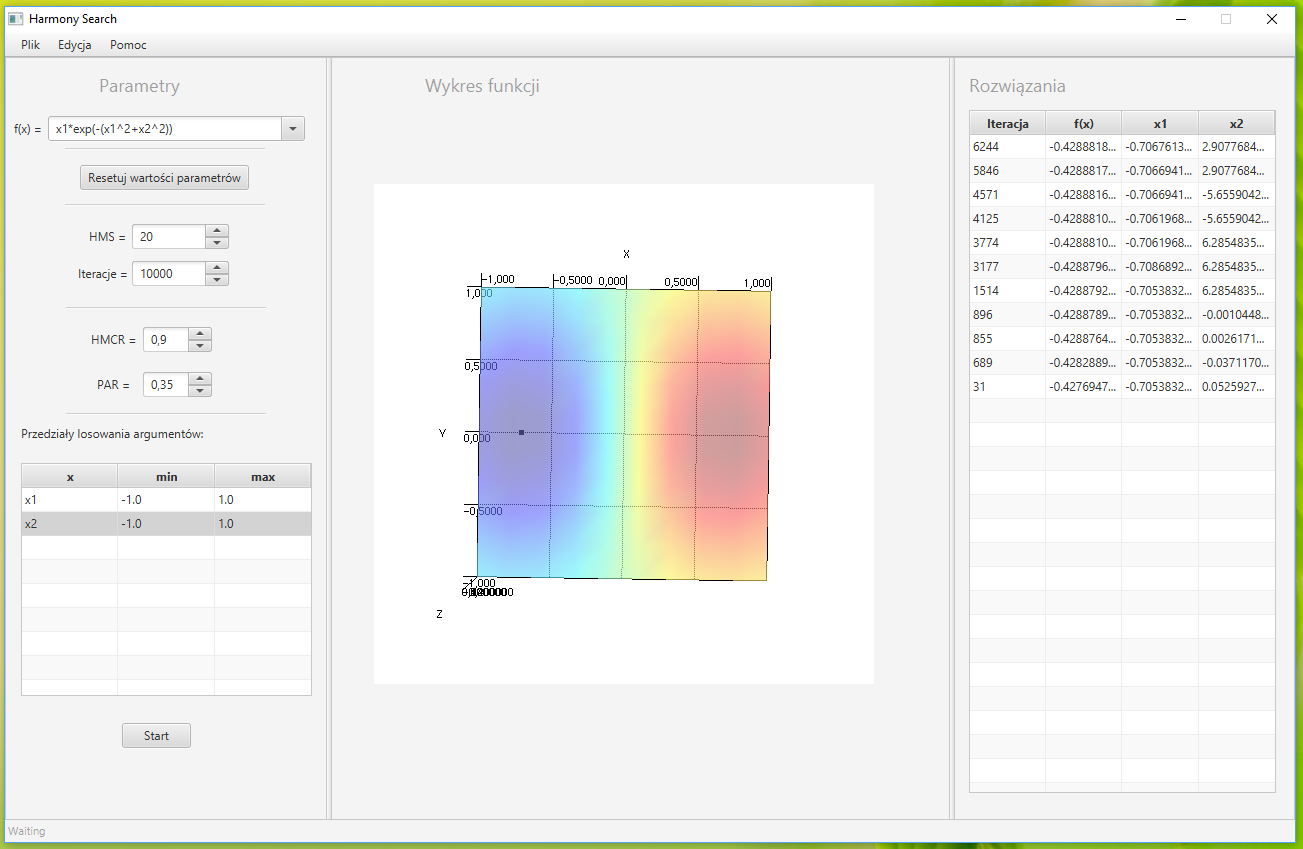
\includegraphics[width=\linewidth]{images/92.PNG} 
	\end{minipage}
	\label{fig:9}
	\caption{Wykres funkcji sinus z eksponentom $x_{1}, x_{2} \in <-1,1>$}
\end{figure}

\subsection{Podsumowanie testów}
\label{subsec:podsumowanietestow}
Sprawdzając działanie algorytmu dla różnych funkcji można stwierdzić, że poprawnie znajduje ich minimum lokalne. Dla funkcji jedno i dwu wymiarowych algorytm działa idealnie. Podczas szukania minimum funkcji trzech zmiennych należy maksymalnie zawęzić obszar. Algorytm działa na tyle szybko, że dla użytkownika nie odczuwalny jest dyskomfort podczas użytkowania programu. Dodatkowo gdy funkcja posiada więcej niż jedno minimum można znaleźć wszystkie z nich zmniejszając przedział dla argumentów. Taka sytuacja została zaprezentowana w punkcie \ref{subsubsec:fcn4min2}. 

\section{Problemy podczas pracy}
\label{sec:problemy}
Jednym z problemów z jakim musiał poradzić sobie program było prezentowanie danych. Algorytm jest zdolny do obliczania funkcji wielu zmiennych dla {\em $x_{n} , n \in N$}. Prezentowanie zmiennych w tabelach jest rzeczą dającą się w prosty sposób rozwinąć. Jednak rysowanie wykresu dla $n \leq 2$ ilości zmiennych nie jest możliwy. Najładniejsze wykresy powstają dla $n = 2$ dlatego funkcje o dwóch zmiennych zostały przedstawione w rozdziale \ref{sec:przyklady}. \\

\section{Wnioski końcowe}
\label{sec:wnioski}
Program obliczający minimum funkcji wielu zmiennych według algorytmu {\em Harmony Search} działa tak jak założono na początku. Spełniły się domniemania na temat szybkości funkcji. Dodatkowo szybkość poprawiła się gdy zamiast zwykłej tablicy dla {\tt HM} przyjęto {\tt SortedSet}. Oczywistym jest, że program najdokładniej przybliży rozwiązanie gdy zakres wartości {\em x} będzie jak najbliższy minimum funkcji. Dodatkowo gdy zmniejszymy ilość iteracji program zakończy szybciej swoje działanie, lecz kosztem gorszego przybliżenia. Gdy wymagane jest obliczenie każdego z minimum funkcji możemy je znaleźć i obliczyć jego wartość o ile znamy przedział, w którym jest ono umiejscowione. 

\newpage
\addcontentsline{toc}{section}{Bibilografia}
\bibliography{bibliografia}
\bibliographystyle{plain}
\end{document}

